% =============================================
% 实验报告 / 课程报告 LaTeX 通用模板
% 基于 xelatex + ctex 编译
% 适用：A4 / 12pt / 中文（宋体 + 黑体）
% =============================================
\documentclass[12pt, a4paper]{article}

% ---- 中文支持 ----
% 注：以下字体路径基于 macOS。若在其他系统上使用，请把 Path=... 替换为本机字体目录
% 或直接删除 Path 与 FontIndex 选项，改用系统已注册的字体名称（如 SimSun、SimHei）。
\usepackage[fontset=none]{ctex}
\setCJKmainfont{Songti.ttc}[Path=/System/Library/Fonts/Supplemental/, FontIndex=3, BoldFont=Songti.ttc, BoldFeatures={FontIndex=3}]
\setCJKsansfont{STHeiti Light.ttc}[Path=/System/Library/Fonts/, BoldFont=STHeiti Light.ttc]
\setCJKmonofont{Songti.ttc}[Path=/System/Library/Fonts/Supplemental/, FontIndex=3, BoldFont=Songti.ttc, BoldFeatures={FontIndex=3}]
\setCJKfamilyfont{zhsong}{Songti.ttc}[Path=/System/Library/Fonts/Supplemental/, FontIndex=3, BoldFont=Songti.ttc, BoldFeatures={FontIndex=3}]
\setCJKfamilyfont{zhhei}{STHeiti Light.ttc}[Path=/System/Library/Fonts/, BoldFont=STHeiti Light.ttc]
\setCJKfamilyfont{zhfs}{Songti.ttc}[Path=/System/Library/Fonts/Supplemental/, FontIndex=3, BoldFont=Songti.ttc, BoldFeatures={FontIndex=3}]
\setCJKfamilyfont{zhkai}{Songti.ttc}[Path=/System/Library/Fonts/Supplemental/, FontIndex=3, BoldFont=Songti.ttc, BoldFeatures={FontIndex=3}]
\setCJKfamilyfont{coverhei}{STHeiti Medium.ttc}[Path=/System/Library/Fonts/]
\newcommand{\songti}{\CJKfamily{zhsong}}
\newcommand{\heiti}{\CJKfamily{zhhei}}
\newcommand{\fangsong}{\CJKfamily{zhfs}}
\newcommand{\kaishu}{\CJKfamily{zhkai}}
\newcommand{\coverhei}{\CJKfamily{coverhei}}

% ---- 页面布局 ----
\usepackage[
  top=2.5cm, bottom=2.5cm,
  left=3cm,  right=2.5cm
]{geometry}

% ---- 图片 ----
\usepackage{graphicx}
\usepackage{float}
\graphicspath{{figures/}}

% ---- 表格 ----
\usepackage{booktabs}
\usepackage{tabularx}
\usepackage{multirow}
\usepackage{colortbl}

% ---- 代码高亮 ----
\usepackage{listings}
\usepackage{xcolor}

\lstset{
  basicstyle=\ttfamily\small,
  keywordstyle=\color{blue}\bfseries,
  commentstyle=\color{gray}\itshape,
  stringstyle=\color{red!70!black},
  numbers=left,
  numberstyle=\tiny\color{gray},
  numbersep=8pt,
  breaklines=true,
  frame=single,
  rulecolor=\color{black!30},
  backgroundcolor=\color{gray!5},
  showstringspaces=false,
  tabsize=4,
}

% ---- 超链接 ----
\usepackage[
  colorlinks=true,
  linkcolor=blue!70!black,
  urlcolor=blue,
  citecolor=green!50!black
]{hyperref}

% ---- 数学 ----
\usepackage{amsmath, amssymb}

% ---- 页眉页脚 ----
\usepackage{fancyhdr}
\pagestyle{fancy}
\fancyhf{}
\fancyhead[L]{\small \courseName}
\fancyhead[R]{\small \leftmark}
\fancyfoot[C]{\thepage}
\renewcommand{\headrulewidth}{0.4pt}
\setlength{\headheight}{14pt}

% ---- 其他工具 ----
\usepackage{enumitem}
\usepackage{caption}
\captionsetup{font=small, labelfont=bf}
\usepackage{subcaption}

% ---- 封面绘图 ----
\usepackage{tikz}
\usetikzlibrary{positioning, arrows.meta, shapes.geometric, fit}
\usepackage{array}

% =============================================
%  封面信息（每次新报告只需修改这一段）
% =============================================
\newcommand{\courseName}{深度学习}                   % 页眉左侧 / 课程名
\newcommand{\expTitle}{期末报告}                     % 封面正中大字
\newcommand{\expFullTitle}{基于 VGGT 场景重建与 TRELLIS\\三维生成的真实场景编辑方法} % 题目栏
\newcommand{\academicYear}{2025-2026-2}              % 学年学期
\newcommand{\college}{计算机学院}
\newcommand{\major}{计算机科学与技术}
\newcommand{\className}{周四8-9}
\newcommand{\studentName}{徐熠潘\hspace{0.22cm}胡鑫园\hspace{0.22cm}夏君旸}
\newcommand{\studentID}{24051133\hspace{0.18cm}24050136\hspace{0.18cm}23050236}
\newcommand{\instructor}{杨艳}
\newcommand{\expDate}{2026 年 6 月}

% 校名图片文件名（位于 figures/ 下，不带路径前缀）
\newcommand{\titleLogo}{hdu_logo_blue.png}

% 缺失实验图片的统一占位框。后续只需用 \includegraphics 替换整个命令。
\newcommand{\figureplaceholder}[3]{%
  \begin{figure}[H]
    \centering
    \fbox{\parbox[c][#1][c]{0.88\linewidth}{%
      \centering\color{gray!70}\heiti
      图片待补充\\[0.5em]
      \normalfont\small #2}}
    \caption{#2}
    \label{#3}
  \end{figure}
}

% =============================================
\begin{document}

% ---- 封面 ----
\begin{titlepage}
  \thispagestyle{empty}

  \begin{tikzpicture}[remember picture,overlay]
    % ---- 校名图片 ----
    \node[inner sep=0pt, anchor=center] at ([yshift=-5.85cm]current page.north)
      {\includegraphics[width=11.95cm]{\titleLogo}};

    % ---- 实验大标题 ----
    \node[anchor=center, font=\coverhei\bfseries\fontsize{28}{34}\selectfont]
      at ([yshift=-9.82cm]current page.north)
      {《\hspace{0.18cm}深\hspace{0.18cm}度\hspace{0.18cm}学\hspace{0.18cm}习\hspace{0.18cm}》};
    \node[anchor=center, font=\coverhei\bfseries\fontsize{28}{34}\selectfont]
      at ([yshift=-11.42cm]current page.north)
      {期\hspace{0.38cm}末\hspace{0.38cm}报\hspace{0.38cm}告};

    % ---- 信息表格 ----
    \coordinate (tableTopLeft) at ([xshift=-4.15cm,yshift=-15.35cm]current page.north);
    \def\coverTableWidth{8.30}
    \def\coverLabelWidth{2.70}
    \def\coverRowHeight{1.40}
    \foreach \row in {0,...,5} {
      \draw[gray!45, line width=0.35pt, dash pattern=on 1pt off 1pt]
        ([yshift=-\row*\coverRowHeight cm]tableTopLeft) --
        ([xshift=\coverTableWidth cm,yshift=-\row*\coverRowHeight cm]tableTopLeft);
    }
    \foreach \x in {0,\coverLabelWidth,\coverTableWidth} {
      \draw[gray!45, line width=0.35pt, dash pattern=on 1pt off 1pt]
        ([xshift=\x cm]tableTopLeft) --
        ([xshift=\x cm,yshift=-5*\coverRowHeight cm]tableTopLeft);
    }
    \foreach \row in {1,...,5} {
      \draw[black, line width=0.45pt]
        ([xshift=\coverLabelWidth cm,yshift=-\row*\coverRowHeight cm]tableTopLeft) --
        ([xshift=\coverTableWidth cm,yshift=-\row*\coverRowHeight cm]tableTopLeft);
    }

    \foreach \label/\value/\row in {
      {姓\hspace{0.62cm}名:}/{\studentName}/0,
      {学\hspace{0.62cm}号:}/{\studentID}/1,
      {学\hspace{0.62cm}院:}/{\college}/2,
      {班\hspace{0.62cm}级:}/{\className}/3,
      {专\hspace{0.62cm}业:}/{\major}/4
    } {
      \node[anchor=center, font=\coverhei\bfseries\fontsize{17}{20}\selectfont]
        at ([xshift=1.35cm,yshift=-\row*\coverRowHeight cm-0.70cm]tableTopLeft) {\label};
      \node[anchor=center, text width=5.45cm, align=center,
        font=\coverhei\bfseries\fontsize{15}{19}\selectfont]
        at ([xshift=5.50cm,yshift=-\row*\coverRowHeight cm-0.70cm]tableTopLeft) {\value};
    }

    % ---- 完成时间 ----
    \node[anchor=center, font=\coverhei\bfseries\fontsize{17}{20}\selectfont]
      at ([yshift=-25.55cm]current page.north)
      {完成时间:\quad
        \underline{\makebox[2.25cm][c]{2026}}\ 年\quad
        \underline{\makebox[1.25cm][c]{6}}\ 月};
  \end{tikzpicture}
  \null

\end{titlepage}

% ---- 目录 ----
\tableofcontents
\newpage

% =============================================
%  正文
%  小提示：
%   - 章节多时可用 \input{sections/01-purpose.tex} 等方式拆分
%   - 图片放 figures/ 下，\includegraphics 时省略路径前缀
%   - 代码块用 lstlisting 环境，已在 \lstset 中预设样式
% =============================================

\section*{\centering 摘要}
\addcontentsline{toc}{section}{摘要}

面向增强现实、数字孪生和三维内容创作的真实场景编辑，需要同时处理两件事：从有限图像中恢复可用的空间结构，并让新增内容具有完整几何、合理外观和跨视角一致性。传统三维重建通常依赖特征匹配、Structure-from-Motion、Bundle Adjustment 和 Multi-View Stereo 等多阶段优化，流程较长，也难以满足交互速度；二维扩散模型虽然语义生成能力强，但逐视图编辑容易引入几何冲突。围绕这一问题，本文完成 Visual Geometry Grounded Transformer（VGGT）与 TRELLIS 两个官方工程的独立复现，并分析二者在真实场景三维融合编辑中的互补关系。

在独立复现之外，本文设计了一套尚未实现的融合编辑流程：使用 VGGT 从教室多视图图像中估计相机参数、深度、pointmap 和置信度，以 TRELLIS 根据文本或参考图像生成三维资产，再通过尺度、旋转和平移完成资产注册，并用地面几何、背景保持和多视图重投影约束候选结果。方案还计划利用 VGGT 置信度、相对位姿漂移和深度/pointmap cycle consistency 对候选编辑进行检查。上述注册、融合、重渲染和闭环评分均属于方法设计，并未在本次实验中实现。

现阶段的实验成果只包括两个基础模型的独立复现：VGGT 已获得多视图深度、相机位姿与场景可视化结果；TRELLIS 已跑通图像/文本条件生成及 mesh、3D Gaussian、Radiance Field 解码流程。当前尚未实现连接两者的统一执行脚本，也没有可作为实验结果报告的融合场景。因此，本文在行文中区分“已完成的模型复现”和“提出但未实现的融合编辑思想”，后者作为后续继续实现的方向。

\vspace{\baselineskip}
\noindent\textbf{关键词：}VGGT；TRELLIS；三维重建；三维生成；场景编辑；多视图一致性

\newpage

\section{绪论}

\subsection{研究背景}

从二维图像恢复三维结构并进一步编辑，是计算机视觉与计算机图形学长期交叉的核心问题。其应用覆盖虚拟现实、增强现实、数字孪生、游戏资产制作、机器人感知和室内空间设计。传统方法通常先利用局部特征建立图像对应关系，通过 Structure-from-Motion（SfM）估计稀疏点云和相机位姿，再通过 Multi-View Stereo（MVS）恢复稠密几何，最后借助 NeRF 或 3D Gaussian Splatting（3DGS）完成新视角合成。该流程具有清晰的几何解释，但多个阶段会累积误差，并且往往需要逐场景优化。

近年来，大规模视觉 Transformer 和三维数据训练推动了前馈三维重建。DUSt3R 将两视图重建改写为 canonical pointmap 回归\cite{dust3r}；VGGT 进一步在一个多视图 Transformer 中联合预测相机、深度、pointmap 和跟踪特征\cite{vggt}，使一张至数百张图像的关键几何属性可以在数秒内获得。与传统管线相比，VGGT 不仅缩短了推理链路，还提供统一世界坐标、跨视图对应关系和像素级置信度，为三维编辑提供了更直接的几何接口。

在三维生成方面，TRELLIS 提出 Structured LATent（SLAT），在稀疏三维网格的 active voxels 上存储局部潜变量，并使用两阶段 rectified flow 分别生成稀疏结构和局部细节\cite{trellis}. 同一潜表示可以解码为 mesh、Radiance Field 或 3D Gaussians，并支持局部区域重采样。由此，VGGT 与 TRELLIS 形成明显互补：前者回答“真实场景在哪里、相机如何观察”，后者回答“需要添加或替换的三维内容如何生成”。

\subsection{问题定义}

本文关注如下任务：给定同一真实场景的多视图图像集合
\begin{equation}
  \mathcal{I}=\{I_i\}_{i=1}^{N},
\end{equation}
以及文本或图像形式的编辑条件 $c$，首先恢复场景几何表示 $\mathcal{G}$，再生成目标三维资产 $\mathcal{A}$，最终通过空间变换 $T=(s,\mathbf{R},\mathbf{t})$ 获得编辑后场景
\begin{equation}
  \mathcal{G}_{\mathrm{edit}}
  =\mathcal{G}\cup T(\mathcal{A}),\qquad
  T(\mathbf{x})=s\mathbf{R}\mathbf{x}+\mathbf{t}.
\end{equation}
这里，$s$、$\mathbf{R}$ 和 $\mathbf{t}$ 分别控制资产尺度、朝向和位置。系统应满足三个要求：生成内容符合语义条件；资产与原场景几何关系合理；编辑结果在多个视角下保持一致。

\subsection{研究内容与主要工作}

本文完成的复现与提出的方法可归纳为三项主要工作：

\begin{enumerate}[label=\arabic*.]
  \item \textbf{统一高斯表示与图文双驱。}完成 VGGT 在真实多视图上的几何输出与可视化验证，并核对 TRELLIS 1 的图像/文本条件、两阶段采样与多格式解码接口。在此基础上，设计以 3DGS 为内部工作表示的统一编辑链路。
  \item \textbf{真实场景融合与语言精确编辑。}设计将 VGGT 的相机位姿、pointmap 与置信度用于场景初始化、空间定位和编辑后验证；结合 REALM 式全局到局部定位、SAM2 二维掩码与多视图三维回投，将语言指令映射为高斯实例选区，并为添加、移动、删除、替换和材质编辑定义可执行算子。
  \item \textbf{高保真多格式交付。}代码审计确认 TRELLIS 1 同一 SLat 可解码为 3DGS、Radiance Field 与 Mesh，VGGT 可导出点云 GLB 与 COLMAP 数据；在此基础上，以 TRELLIS 2 的 O-Voxel 作为后续保留复杂几何和 PBR 材质的扩展方向。
\end{enumerate}

\subsection{报告结构}

第 2 节梳理前馈三维重建、三维生成与编辑相关工作；第 3 节介绍 VGGT、TRELLIS 和 3DGS 等理论基础；第 4 节给出融合系统的方法设计；第 5 节以源码为依据说明两个工程的实际接口、导出格式与实现边界；第 6 节展示已验证结果并给出融合实验的实现状态和评价设计；第 7 节总结工作并讨论后续方向。

\section{相关工作}

\subsection{从 DUSt3R 到 VGGT 的前馈三维重建}

DUSt3R 不再把相机标定视为稠密重建的前置条件，而是从一对图像直接回归表达在第一相机坐标系中的两个 pointmap\cite{dust3r}。该表示同时保存像素到三维点的映射和两视图间的几何关系，并可恢复焦距、相对位姿和像素匹配。对于多视图输入，DUSt3R 仍需把多组 pairwise pointmap 通过全局优化对齐，因此推理时间和误差传播仍受到图像对数量影响。

VGGT 将上述范式扩展到任意数量图像。模型以第一相机为参考坐标系，通过交替的帧内注意力和全局注意力联合推理所有视图，同时输出相机、深度、pointmap 与跟踪特征\cite{vggt}。对于本文的编辑任务，VGGT 的价值主要在于把相机、稠密几何和跟踪信息放入同一套特征中，而不只是提高某个深度指标。CUT3R 通过持久状态支持在线图像流和未观测视角查询\cite{cut3r}；Easi3R 从 DUSt3R cross-attention 中分解动态区域，在不重新训练的条件下改善动态 4D 重建\cite{easi3r}；VGGT-$\Omega$ 则以 scene registers、register attention、轻量 dense head 和大规模自监督扩展模型容量及动态泛化\cite{vggtomega}。

\subsection{可渲染三维表示}

pointmap 适合表达像素对齐几何，却不直接包含用于高质量渲染的 opacity、scale、rotation 和 view-dependent appearance。3DGS 将场景表示为一组三维高斯，每个高斯包含中心 $\boldsymbol{\mu}$、协方差 $\boldsymbol{\Sigma}$、不透明度 $\alpha$ 与球谐颜色系数，通过可微 splatting 实现实时渲染\cite{3dgs}。FLARE 采用位姿估计、相机局部几何、全局几何投影和 Gaussian head 级联结构，从无标定稀疏视图直接预测可渲染三维场景\cite{flare}。这说明从 VGGT pointmap 到 3DGS 仍需进行尺度、局部表面和外观参数建模。

\subsection{原生三维生成}

TRELLIS 通过 SLAT 在 active voxels 上联合表达粗结构与局部几何/外观，使用 DINOv2 多视图特征和 sparse VAE 学习统一潜空间，再以两个 rectified-flow Transformers 依次生成稀疏结构和局部潜变量\cite{trellis}。该设计可以解码到多种三维格式，也允许固定未编辑区域、只重采样局部潜变量。TRELLIS 2 进一步提出 field-free 的 O-Voxel，将任意拓扑几何与 PBR 材质压缩到紧凑潜空间，以处理开放表面、非流形结构、内部表面和透明材质\cite{trellis2}。SynCity 则利用 LLM、二维生成器和 TRELLIS 逐 tile 构建可导航世界，给出了对象级生成器向大场景扩展的一种做法\cite{syncity}。

\subsection{文本驱动三维编辑}

现有三维编辑大体可分为三类。第一类在原生三维几何中预测局部变化。VGGT-Edit 将编辑写成 edit mask 内的稠密残差位移场，并通过文本分层注入、视图权重、法向一致和背景保持约束降低跨视图冲突\cite{vggtedit}。需要注意的是，该工作冻结的是 $\pi^3$ 重建骨干，并非直接在原版 VGGT 权重上增加编辑头，但其 pointmap 残差思想可迁移到 VGGT 输出。

第二类保留二维编辑模型的强语义能力，再使用三维模型验证一致性。RL3DEdit 使用 FLUX-Kontext 联合编辑多个视图，并把 VGGT 的深度/point confidence 和相对位姿误差作为 GRPO 奖励\cite{rl3dedit}。这说明直接生成三维一致的多视图内容较难，但利用几何模型识别矛盾相对可行。

第三类采用 agent 编排多个工具。REALM 通过 3DGS feature field 与 Global-to-Local Spatial Grounding，将隐式语言指令转成精细三维 mask\cite{realm}；Vinedresser3D 使用 MLLM 解析增加、修改和删除指令，通过 PartField 定位三维区域，再交替调用 TRELLIS-text 与 TRELLIS-image 完成潜空间反演编辑\cite{vinedresser}. TwinTex 虽不属于 VGGT 路线，但其中的平面视图选择、结构线对齐和扩散纹理补全，对教室墙面、地面等规则区域仍有参考意义\cite{twintex}。

\subsection{本文定位}

与需要大规模训练的 VGGT-Edit 和 RL3DEdit 不同，本文以本地已部署的 VGGT 与 TRELLIS 1 官方代码为基础，优先研究无需重新训练基础模型的系统组合：VGGT 提供真实空间与几何约束，TRELLIS 提供新增内容，显式相似变换负责连接两者。当前仓库尚未实现这一连接层，因此本文重点放在可执行数据接口、误差来源，以及后续语义 grounding、残差编辑与 VGGT verifier 的实现边界上。

\section{模型原理与技术基础}

\subsection{VGGT 的多视图统一几何预测}

设输入为 $N$ 张观察同一场景的 RGB 图像，VGGT 学习映射
\begin{equation}
  f\left(\{I_i\}_{i=1}^{N}\right)
  =\{g_i,D_i,P_i,F_i,\Sigma_i\}_{i=1}^{N},
\end{equation}
其中 $g_i$ 表示相机内外参，$D_i$ 表示深度，$P_i$ 表示在第一相机坐标系下的 viewpoint-invariant pointmap，$F_i$ 表示跟踪特征，$\Sigma_i$ 表示预测不确定性。给定像素齐次坐标 $\tilde{\mathbf{u}}=[u,v,1]^\top$，深度与相机可以反投影为
\begin{equation}
  \mathbf{x}_{i}^{(c)}=D_i(u,v)\mathbf{K}_i^{-1}\tilde{\mathbf{u}},
  \qquad
  \mathbf{x}_{i}^{(w)}=\mathbf{R}_i^\top
  \left(\mathbf{x}_{i}^{(c)}-\mathbf{t}_i\right).
\end{equation}

VGGT 使用 DINO 将图像分块为视觉 token，并追加 camera token 与 register token。其主干不是持续执行昂贵的全局注意力，而是交替采用两种注意力：frame-wise self-attention 在每幅图内部更新局部结构，global self-attention 在所有视图间建立对应和全局几何。第一帧使用特殊 token 以确定参考坐标，除第一帧外的图像顺序保持排列等变。

图 \ref{fig:vggt-paper-pipeline} 展示了 VGGT 的完整前馈路径。不同颜色表示来自不同输入图像的 token；全局注意力负责跨视图交换信息，帧内注意力则在各自图像内部更新局部表征。经过多层交替注意力后，camera token 进入 Camera Head，图像 token 进入 DPT dense prediction head，分别产生相机、深度、pointmap 和跟踪结果。这种共享主干、多任务分头预测的结构，使相机估计与稠密几何能够相互提供约束。

\begin{figure}[htbp]
  \centering
  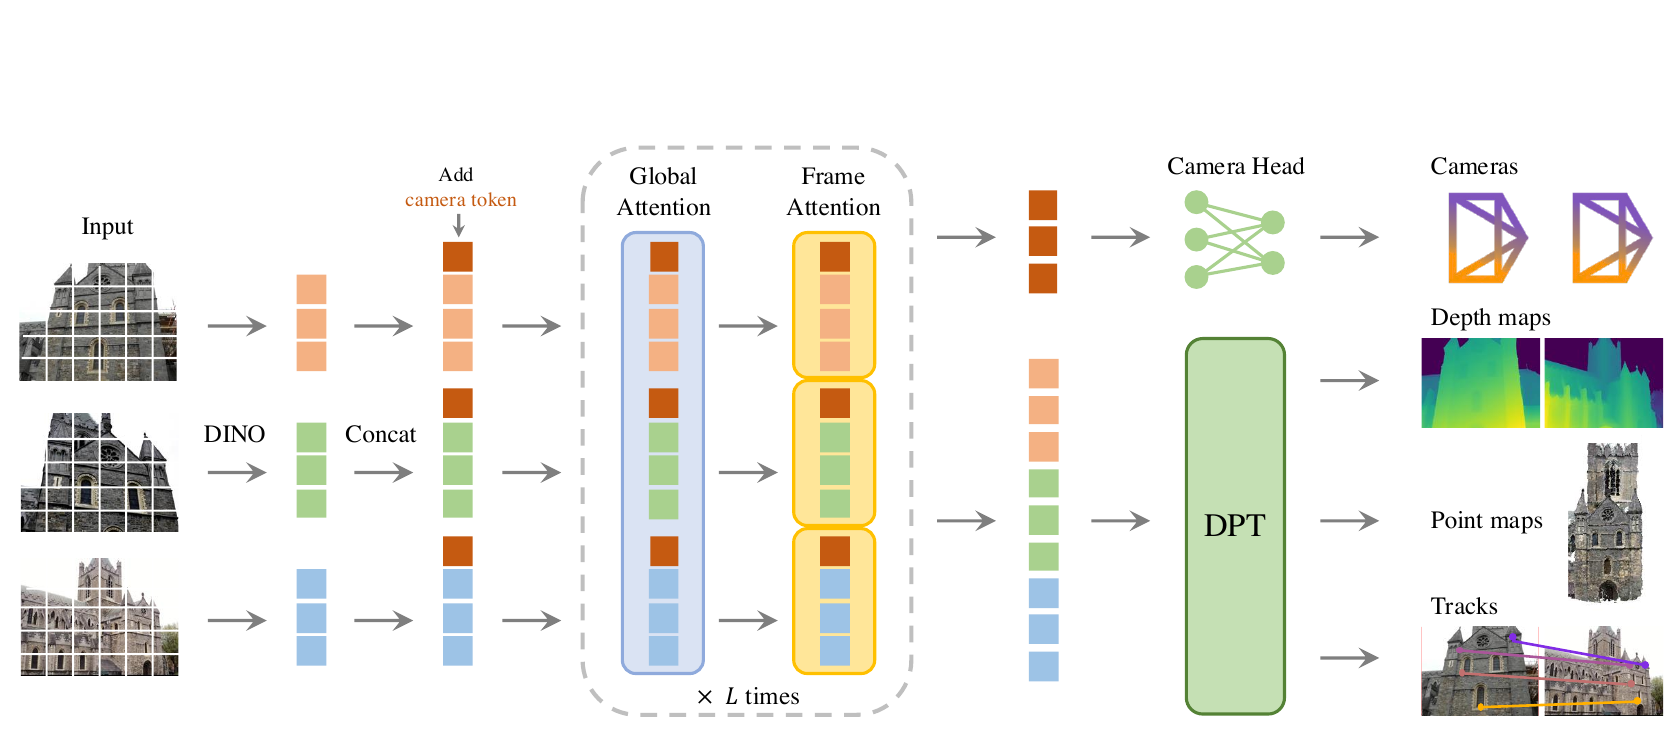
\includegraphics[width=0.98\linewidth]{paper_vggt_pipeline.png}
  \caption{VGGT 整体架构，包括 DINO 图像编码、交替注意力及多任务预测头（引自文献 \cite{vggt} 的 Fig. 2）}
  \label{fig:vggt-paper-pipeline}
\end{figure}

VGGT 同时监督相机、深度、pointmap 与 tracking。尽管这些量存在解析关系，过完备的多任务监督能促使主干学习更可靠的三维表示。推理时可根据具体任务选择直接 pointmap，或由相机与深度重新反投影。对于编辑系统，后者便于控制尺度、过滤低置信区域并建立统一三维坐标。

\subsection{TRELLIS 的 Structured LATent}

对于三维资产 $O$，TRELLIS 将其表示为
\begin{equation}
  z=\{(\mathbf{z}_i,\mathbf{p}_i)\}_{i=1}^{L},
  \qquad
  \mathbf{p}_i\in\{0,1,\ldots,N-1\}^3,
\end{equation}
其中 $\mathbf{p}_i$ 是与物体表面相交的 active voxel 位置，$\mathbf{z}_i$ 是对应局部潜变量。由于 $L\ll N^3$，模型可以在高空间分辨率下避免处理大量空体素。active voxel 描述粗结构，局部 latent 记录精细形状和外观。

SLAT 的学习分为编码和解码。首先从多个视角渲染资产，用 DINOv2 抽取二维特征，并将其投影聚合到 active voxels；随后 sparse VAE 把体素特征编码到结构化潜空间。不同 decoder 可以将同一潜变量解码成 mesh、Radiance Field 或 3D Gaussian。生成时，第一阶段 flow model 预测 sparse structure，第二阶段只在 active cells 上预测 local latents。

如图 \ref{fig:trellis-paper-pipeline} 所示，TRELLIS 同时包含“资产编码与解码”和“条件生成”两条路径。上半部分把多视图 DINOv2 特征与稀疏结构融合，经 Sparse VAE 得到 SLAT，并通过不同 decoder 输出 3DGS、Radiance Field 或 mesh；下半部分先生成 sparse structure，再在非空位置生成 structured latents，最后解码为目标三维格式。两阶段生成将全局拓扑与局部细节分开建模，是 TRELLIS 能够进行区域级重采样和局部编辑的基础。

\begin{figure}[htbp]
  \centering
  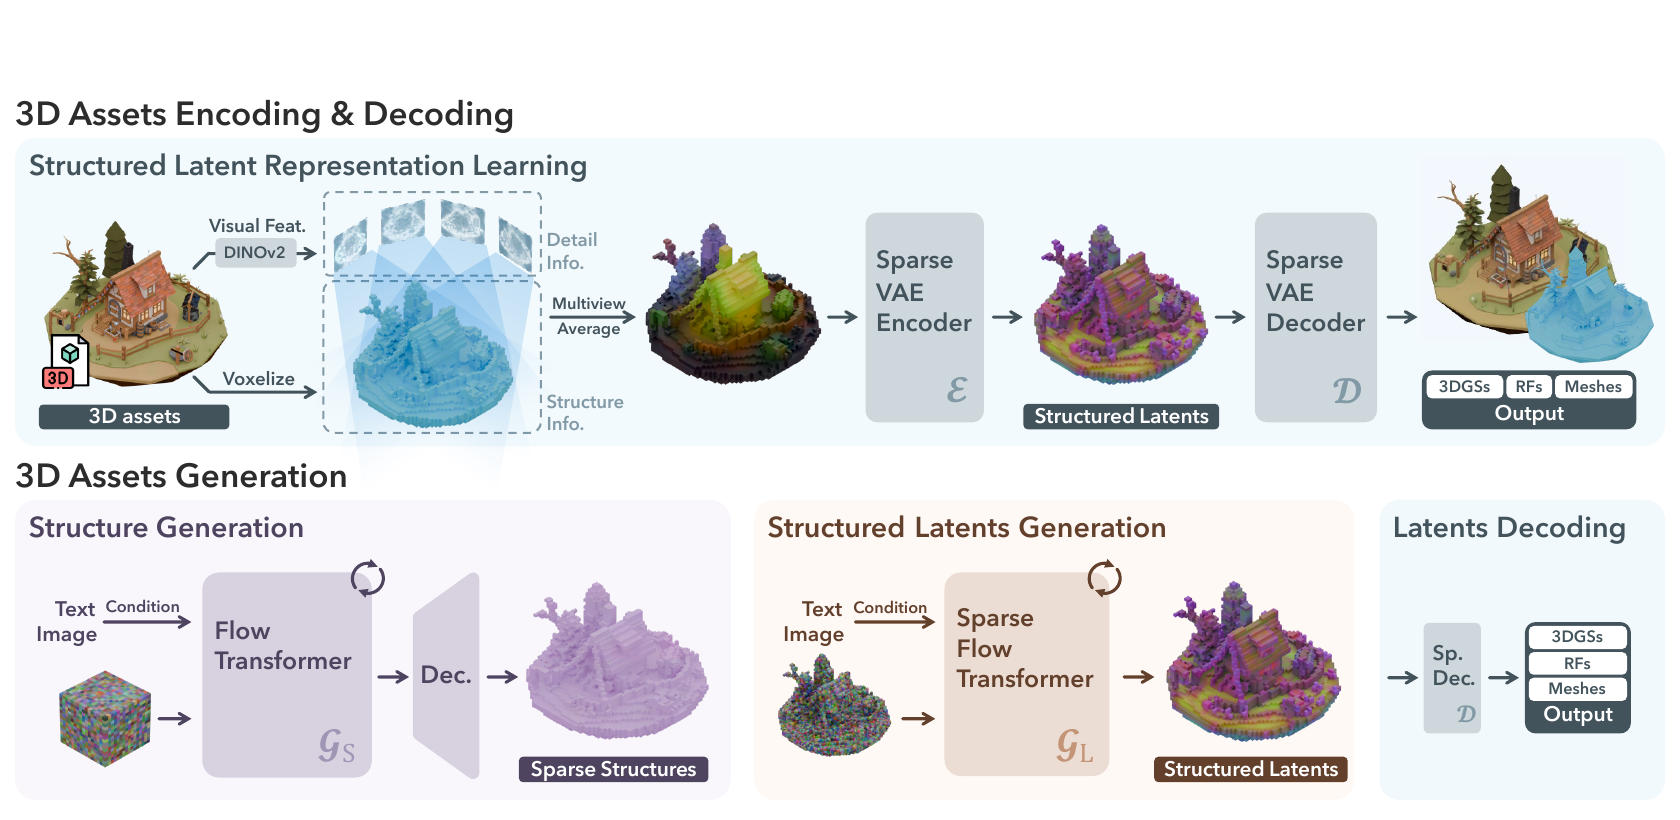
\includegraphics[width=0.98\linewidth]{paper_trellis_pipeline.png}
  \caption{TRELLIS 的 SLAT 编码、两阶段生成与多格式解码流程（引自文献 \cite{trellis} 的 Fig. 2）}
  \label{fig:trellis-paper-pipeline}
\end{figure}

Rectified flow 使用数据样本 $\mathbf{x}_0$ 与噪声 $\boldsymbol{\epsilon}$ 的线性路径
\begin{equation}
  \mathbf{x}(t)=(1-t)\mathbf{x}_0+t\boldsymbol{\epsilon},
\end{equation}
并学习速度场 $v_\theta(\mathbf{x},t)$：
\begin{equation}
  \mathcal{L}_{\mathrm{CFM}}
  =\mathbb{E}_{t,\mathbf{x}_0,\boldsymbol{\epsilon}}
  \left\|v_\theta(\mathbf{x},t)-(\boldsymbol{\epsilon}-\mathbf{x}_0)\right\|_2^2.
\end{equation}
两阶段解耦使 TRELLIS 能固定结构只改变细节，或给定三维 bounding box 对局部结构和潜变量进行 RePaint 式重采样。

\subsection{3D Gaussian Splatting}

一个三维 Gaussian 可记为
\begin{equation}
  G_k=(\boldsymbol{\mu}_k,\mathbf{R}_k,\mathbf{s}_k,
  \alpha_k,\mathbf{c}_k),
\end{equation}
其中 $\boldsymbol{\mu}_k$ 为中心，$\mathbf{R}_k$ 与 $\mathbf{s}_k$ 决定协方差
\begin{equation}
  \boldsymbol{\Sigma}_k
  =\mathbf{R}_k\operatorname{diag}(\mathbf{s}_k^2)\mathbf{R}_k^\top.
\end{equation}
Gaussian 投影到图像平面后按深度排序并进行 alpha compositing。3DGS 同时具有显式空间位置、实时渲染和可微优化能力，因此适合承担本文的场景编辑表示：对象移动可直接修改 $\boldsymbol{\mu}$，缩放和旋转可修改 $\mathbf{s}$ 与 $\mathbf{R}$，外观编辑可限制在 mask 内更新 opacity 与球谐颜色系数。

从前馈几何到可渲染 Gaussian 的连接可以参考 FLARE。图 \ref{fig:flare-paper-pipeline} 中，网络先从无标定稀疏视图估计粗位姿，在相机坐标系中预测局部几何，再利用细化位姿和 Global Geometry Projector 得到统一点图，最后回归 Gaussian 参数。该流程说明 pointmap 只确定 Gaussian 中心的几何基础；若要得到高质量可渲染场景，还需要从图像特征预测尺度、旋转、不透明度和外观参数。

\begin{figure}[htbp]
  \centering
  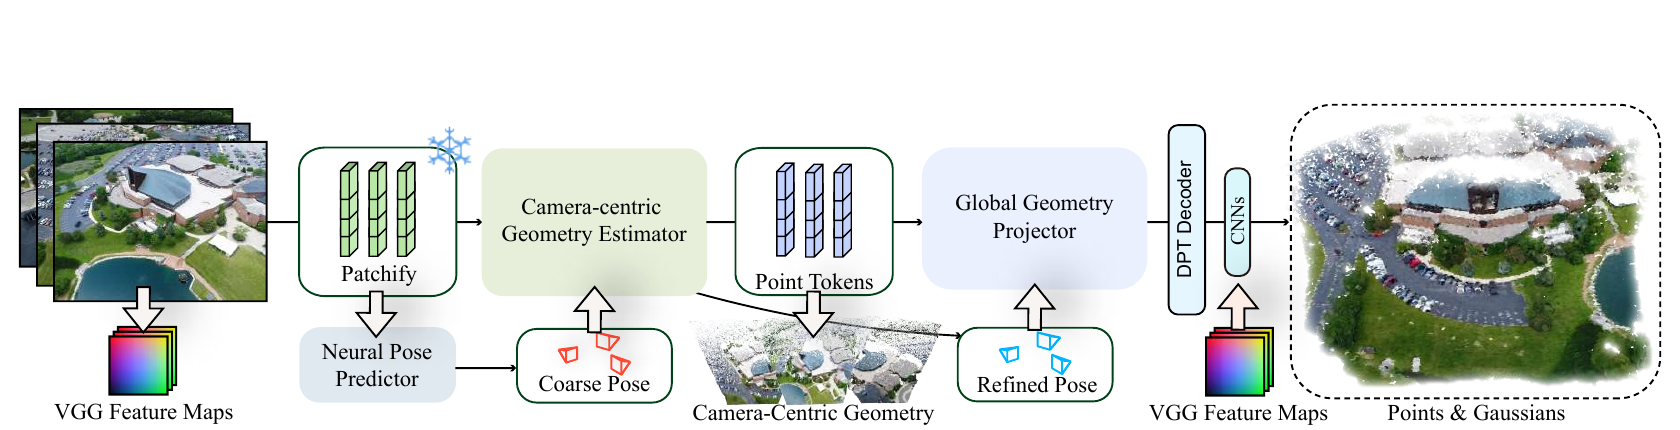
\includegraphics[width=0.98\linewidth]{paper_flare_pipeline.png}
  \caption{FLARE 从稀疏无标定视图到全局点图与 3D Gaussians 的前馈管线（引自文献 \cite{flare} 的 Fig. 2）}
  \label{fig:flare-paper-pipeline}
\end{figure}

\subsection{重建与生成的互补关系}

VGGT 输出的是以输入观测为依据的场景几何，优势是相机和多视图对应可靠，但无法凭空生成完整新资产；TRELLIS 学习三维资产分布，可以补充不可见面并生成新对象，但其局部坐标、尺度和朝向不属于真实场景。本文使用显式空间对齐连接二者：VGGT 决定“放在哪里”，TRELLIS 决定“生成什么”，3DGS 或 mesh 决定“如何表示和渲染”。

\section{融合 VGGT 与 TRELLIS 的三维场景编辑方法设计}

\noindent\textbf{实现边界说明：}本章提出的是三维融合编辑思想及其工程化设计，不是本次实验已经实现的系统。当前工作仅完成 VGGT 与 TRELLIS 的独立复现；下文涉及的场景注册、语言定位、局部融合、多视图重渲染和 VGGT 闭环评分均为待实现模块，也是后续工作的主要内容。

\subsection{问题定义}

给定同一真实场景的 $N$ 张无标定 RGB 图像
$\mathcal{I}=\{I_i\}_{i=1}^{N}$，以及描述待生成对象的文本或参考图像条件 $c$，
本文设想在不重新训练 VGGT 与 TRELLIS 的前提下，生成编辑后的三维场景
$\mathcal{S}'$。编辑指令可进一步表示为
$q=(o,r,a)$，其中 $o$ 表示操作类型，$r$ 表示目标空间区域，$a$ 表示对象类别、
尺度或朝向等属性。本文重点研究对象添加，并将刚体变换、对象替换与局部补全作为
同一框架下的扩展操作。

该问题的关键并非分别获得一个重建结果和一个生成结果，而是建立二者之间的空间与
评价接口。VGGT 从观测图像恢复场景几何
\begin{equation}
  \mathcal{G}
  =f_{\mathrm{VGGT}}(\mathcal{I})
  =\{\mathbf{K}_i,\mathbf{T}_i,D_i,P_i,C_i\}_{i=1}^{N},
\end{equation}
其中 $\mathbf{K}_i$、$\mathbf{T}_i$、$D_i$、$P_i$ 和 $C_i$ 分别为相机内参、
外参、深度、pointmap 与几何置信度。TRELLIS 根据条件 $c$ 生成局部坐标系中的
三维资产
\begin{equation}
  \mathcal{A}=f_{\mathrm{TRELLIS}}(c),
  \qquad \mathcal{A}\in\{\text{mesh},\text{3DGS},\text{radiance field}\}.
\end{equation}
拟议的融合模块需要求解从资产坐标系到 VGGT 世界坐标系的相似变换
\begin{equation}
  \mathcal{T}_{a\rightarrow w}(\mathbf{x})
  =s\mathbf{R}\mathbf{x}+\mathbf{t},
  \qquad s>0,\quad \mathbf{R}\in \mathrm{SO}(3),
\end{equation}
并使融合结果同时满足语义正确、空间接触合理、多视图几何一致和未编辑区域稳定四类
要求。由此，本文将三维编辑写为候选变换搜索问题：
\begin{equation}
  \mathcal{T}^{*}
  =\arg\max_{\mathcal{T}\in\Omega(r)}
  S\!\left(\operatorname{Fuse}
  (\mathcal{S},\mathcal{T}(\mathcal{A})),q\right),
\end{equation}
其中 $\Omega(r)$ 是由目标区域与支撑平面约束得到的可行变换集合，$S$ 是包含
VGGT 几何反馈的联合评分函数。

\subsection{方法总览}

拟议框架如图 \ref{fig:pipeline} 所示，由统一场景重建、语言定位、条件生成、空间注册、
局部融合和闭环验证六个阶段组成。首先，VGGT 将多视图图像映射到统一参考坐标系，
联合估计相机位姿、深度、pointmap 与几何置信度，并为 3DGS 优化提供相机和高斯中心
初值。对于“删除讲台旁的椅子”或“把桌上的台灯换成绿色植物”等指令，多模态大模型
先在全局视图中解析目标、空间关系、操作类型与保护区域，再在代表视图中输出目标框；SAM2
生成像素级掩码，经多视图可见性和实例特征聚合后得到三维高斯掩码。若指令需要新内容，
TRELLIS 以文本或参考图像为条件生成 mesh 或 3DGS 资产。后续待实现的融合模块再利用场景支撑面、目标包围盒
和几何置信度初始化相似变换，对插入资产及其边界邻域执行局部可微优化。最后，每个编辑候选
沿原相机位姿重新渲染，由 VGGT 置信度、相对位姿、深度循环误差与背景保持项共同排序。

\begin{figure}[htbp]
  \centering
  \resizebox{0.98\linewidth}{!}{%
  \begin{tikzpicture}[
    node distance=1.05cm and 0.68cm,
    box/.style={draw, rounded corners, align=center, minimum height=1.05cm, minimum width=2.45cm, fill=blue!6},
    op/.style={draw, rounded corners, align=center, minimum height=1.05cm, minimum width=2.55cm, fill=orange!10},
    resultbox/.style={draw, rounded corners, align=center, minimum height=1.05cm, minimum width=2.45cm, fill=green!10},
    arr/.style={-{Latex[length=2.3mm]}, thick}
  ]
    \node[box] (images) {真实场景\\多视图图像};
    \node[box, right=of images] (vggt) {VGGT\\统一几何推理};
    \node[resultbox, right=of vggt] (geometry) {相机、深度\\点图、置信度};

    \node[box, below=of images] (condition) {自然语言指令\\文本或参考图像};
    \node[box, right=of condition] (grounding) {MLLM + SAM2\\全局到局部定位};
    \node[resultbox, right=of grounding] (mask) {多视图二维掩码\\三维高斯掩码};

    \node[box, below=of condition] (trellis) {TRELLIS\\条件三维生成};
    \node[resultbox, right=of trellis] (asset) {Mesh / 3DGS\\局部坐标资产};

    \node[op, right=1.0cm of geometry] (register) {支撑面估计与注册\\$s,\mathbf{R},\mathbf{t}$};
    \node[op, below=of register] (candidate) {候选融合与渲染\\$\{\mathcal{S}'_k\}_{k=1}^{K}$};
    \node[op, right=of candidate] (verify) {VGGT 几何闭环\\物理与语义评分};
    \node[resultbox, above=of verify] (output) {最优编辑场景\\$\mathcal{S}'$};

    \draw[arr] (images)--(vggt);
    \draw[arr] (vggt)--(geometry);
    \draw[arr] (condition)--(grounding);
    \draw[arr] (grounding)--(mask);
    \draw[arr] (condition)--(trellis);
    \draw[arr] (trellis)--(asset);
    \draw[arr] (geometry)--(register);
    \draw[arr] (mask)--(register);
    \draw[arr] (asset)--(register);
    \draw[arr] (register)--(candidate);
    \draw[arr] (candidate)--(verify);
    \draw[arr] (verify)--(output);
    \draw[arr, dashed] (verify) to[bend left=20] (register);
  \end{tikzpicture}}
  \caption{融合 VGGT 与 TRELLIS 的训练自由三维场景编辑框架}
  \label{fig:pipeline}
\end{figure}

该设计借鉴了四类参考工作，但对其功能进行了适合课程实验规模的重新组合。VGGT
提供统一相机与稠密几何接口\cite{vggt}；TRELLIS
提供原生三维生成潜空间\cite{trellis}；Vinedresser3D 将复杂编辑分解为条件生成、
区域定位和局部三维生成\cite{vinedresser}；REALM 提供从语言推理到三维高斯实例的
全局到局部定位思路\cite{realm}；RL3DEdit 则证明 VGGT 的几何输出可作为
多视图一致性验证信号\cite{rl3dedit}。与需要大规模成对编辑数据或强化学习训练的方案
不同，本文设计为冻结两个基础模型，仅在推理阶段搜索和筛选空间变换，因此模块边界清楚，
也便于分别分析重建误差、生成误差与注册误差。

\subsection{统一 3DGS 工作表示与 VGGT 场景初始化}

为使真实重建结果、生成资产和语言编辑共用同一渲染器与操作算子，本文将系统内部
工作格式统一为 3D Gaussian Splatting。一个场景表示为
\begin{equation}
  \mathcal{G}=\{G_j\}_{j=1}^{J},\qquad
  G_j=(\boldsymbol{\mu}_j,\boldsymbol{\Sigma}_j,
  \mathbf{c}_j,\alpha_j,\mathbf{f}_j),
\end{equation}
其中 $\boldsymbol{\mu}_j$ 与 $\boldsymbol{\Sigma}_j$ 描述位置、尺度和朝向，$\mathbf{c}_j$ 为颜色或球谐系数，
$\alpha_j$ 为不透明度，$\mathbf{f}_j$ 是用于语义定位的可选实例特征。对像素 $\mathbf{u}$，按深度
排序后的可微 $\alpha$ 混合为
\begin{equation}
  \hat I(\mathbf{u})=\sum_{j\in\mathcal{N}(\mathbf{u})}
  \mathbf{c}_j\,a_j(\mathbf{u})
  \prod_{l<j}\bigl(1-a_l(\mathbf{u})\bigr).
\end{equation}
因此，选中、移动、删除、复制、替换和局部外观调整都可被归结为对一组高斯参数的显式操作。

LiSee 原方案使用 SfM 相机位姿和稀疏点云初始化真实场景。本文将这一环节替换为 VGGT：
相机头提供 $\{\mathbf K_i,\mathbf T_i\}$，dense heads 提供深度、pointmap 和置信度；通过置信筛选的
pointmap 或深度反投影点初始化高斯中心，颜色由对应像素赋值，尺度由局部点间距估计。随后以
VGGT 位姿渲染输入视图，优化高斯的位置、协方差、颜色与不透明度：
\begin{equation}
  \Theta_{\mathrm{real}}^{*}=\arg\min_{\Theta}
  \sum_{i=1}^{N}\omega_i\left[
  \lambda_1\|R_{\Theta}(\mathbf K_i,\mathbf T_i)-I_i\|_1
  +\lambda_s\bigl(1-\operatorname{SSIM}(R_{\Theta},I_i)\bigr)
  \right],
\end{equation}
其中 $\omega_i$ 由该视图的平均几何置信度给定。这里 VGGT 不被误写为直接产生完整 3DGS 外观
参数的模型；它的关键作用是联合估计相机与稠密几何，减少传统“特征匹配--SfM--三角化”链路的
累积误差，再为可渲染高斯场景提供高质量几何初值。

\subsection{基于 VGGT 的场景几何代理}

\subsubsection{置信度感知的多视图融合}

VGGT 的 pointmap 已处于第一相机定义的共同坐标系中，因此无需像逐图像对方法一样
额外执行全局点云配准。对第 $i$ 个视图中的像素 $\mathbf{u}=(u,v)$，本文定义有效性
掩码
\begin{equation}
  M_i(\mathbf{u})=
  \mathbb{I}\!\left[C_i(\mathbf{u})>\tau_c\right]
  \mathbb{I}\!\left[D_{\min}<D_i(\mathbf{u})<D_{\max}\right],
\end{equation}
并构造带颜色与置信权重的场景点集
\begin{equation}
  \mathcal{P}
  =\bigcup_{i=1}^{N}
  \left\{
  \big(P_i(\mathbf{u}),I_i(\mathbf{u}),C_i(\mathbf{u})\big)
  \;\middle|\;M_i(\mathbf{u})=1
  \right\}.
\end{equation}
对于落入同一体素的重复观测，位置与颜色使用置信度加权平均，体素权重则累加不同
视图的可见次数。该步骤同时降低点数和随机 floaters 对平面估计的影响。若使用由
深度反投影得到的点图，则根据 $\mathbf{K}_i$ 和 $\mathbf{T}_i$ 将其变换到相同坐标系，
再执行同样的融合操作。

\subsubsection{目标位置与支撑平面估计}

用户可直接在三维视图指定目标点，也可在某一输入视图中点击像素 $\mathbf{u}_r$。
后者通过 pointmap 得到初始三维位置
\begin{equation}
  \mathbf{p}_0=P_r(\mathbf{u}_r).
\end{equation}
若该点在其他视图中具有有效跟踪对应 $\mathbf{u}_{i}$，则使用置信度加权的几何中值
减弱单视图深度误差：
\begin{equation}
  \mathbf{p}
  =\arg\min_{\mathbf{x}}
  \sum_{i\in\mathcal{V}(r)}
  C_i(\mathbf{u}_i)\left\|\mathbf{x}-P_i(\mathbf{u}_i)\right\|_2.
\end{equation}

对于需要放置在地面或桌面的对象，在 $\mathbf{p}$ 邻域内以 RANSAC 拟合候选平面
\begin{equation}
  \pi:\;\mathbf{n}^{\top}\mathbf{x}+d=0,
  \qquad \|\mathbf{n}\|_2=1.
\end{equation}
平面选择不仅依据内点数，还同时考虑置信度、空间覆盖以及法向稳定性：
\begin{equation}
  Q(\pi)=
  \frac{1}{|\mathcal{N}_{\pi}|}
  \sum_{j\in\mathcal{N}_{\pi}}C_j
  +\lambda_{a}\frac{A(\mathcal{N}_{\pi})}{A_{\mathrm{roi}}}
  -\lambda_{n}\big(1-|\mathbf{n}^{\top}\mathbf{g}|\big),
\end{equation}
其中 $\mathcal{N}_{\pi}$ 为平面内点集合，$A(\cdot)$ 表示其投影覆盖面积，
$\mathbf{g}$ 为估计重力方向。对墙面安装类对象可相应放宽最后一项，并将目标法向改为
局部墙面法向。

\subsection{语言驱动的全局到局部三维定位}

\subsubsection{指令解析与代表视图选择}

参考 REALM 的 Global-to-Local Spatial Grounding 思路\cite{realm}，系统不直接要求用户在三维界面
精确框选。给定指令 $q$ 和由场景渲染的多视图 $\{I_i^R\}$，MLLM 首先输出结构化编辑计划
\begin{equation}
  \Pi_q=(o,\,d_{\mathrm{src}},\,d_{\mathrm{tgt}},\,r,\,h,\,\mathcal{V}_q),
\end{equation}
其中 $o$ 为添加、移动、删除、复制、替换、材质或结构编辑，$d_{\mathrm{src}}$ 与
$d_{\mathrm{tgt}}$ 分别描述编辑前后的对象，$r$ 是空间关系，$h$ 是需要保护的部件或区域，
$\mathcal{V}_q$ 是能清晰观察目标的代表视图集。对每个 $i\in\mathcal{V}_q$，模型返回
\begin{equation}
  (B_i,C_i,E_i)=\operatorname{MLLM}(I_i^R,q),
\end{equation}
即目标框、类别与定位解释。先做场景级推理，再进入局部像素分割，可区分“窗边的椅子”与
“门边的椅子”等同类实例，也为后续的保护区域约束提供语义边界。

\subsubsection{SAM2 掩码的多视图三维回投}

SAM2 以 $B_i$ 为提示生成二维掩码 $M_i^{2D}$。仅用单视图掩码反投影会把遮挡后方或几何噪声
选入目标，因此本文在多视图中聚合每个高斯对掩码像素的渲染贡献。记
\begin{equation}
  w_{ij}(\mathbf{u})=a_{ij}(\mathbf{u})
  \prod_{l<j}\bigl(1-a_{il}(\mathbf{u})\bigr)
\end{equation}
为第 $j$ 个高斯在视图 $i$ 的像素 $\mathbf{u}$ 上经可见性处理后的混合权重，则其三维目标分数为
\begin{equation}
  s_j(q)=
  \frac{\sum_{i\in\mathcal{V}_q}\sum_{\mathbf{u}}
  C_i(\mathbf{u})M_i^{2D}(\mathbf{u})w_{ij}(\mathbf{u})}
  {\sum_{i\in\mathcal{V}_q}\sum_{\mathbf{u}}
  C_i(\mathbf{u})w_{ij}(\mathbf{u})+\varepsilon}.
\end{equation}
其中 $C_i(\mathbf{u})$ 复用 VGGT 几何置信度，使弱纹理、反射或边界区域的错误回投寱减。同时将每个高斯
的实例特征 $\mathbf f_j$ 按同样的 $\alpha$ 混合方式渲染为二维特征图，并与 MLLM 类别描述计算语义
相似度，用于排除遮挡但投影重叠的其他实例。最终三维选区为
\begin{equation}
  \mathcal{M}_q^{3D}=\{G_j\in\mathcal{G}_{\mathrm{real}}
  \mid s_j(q)>\tau_s,\ n_j^{\mathrm{vis}}\geq m\}.
\end{equation}
对非高斯场景表示，也可先用 VGGT pointmap 将 $M_i^{2D}$ 中的像素回投为三维点，再与 mesh face 或
高斯中心做近邻关联。这使 VGGT 同时参与场景生成、相机位姿估计和二维结果的三维落点。

\subsection{TRELLIS 资产生成与规范化}

TRELLIS 的两阶段生成过程可写为
\begin{equation}
  \mathcal{O}\sim G_S(c),\qquad
  \mathbf{z}\sim G_L(\mathcal{O},c),\qquad
  \mathcal{A}=D_{\rho}(\mathcal{O},\mathbf{z}),
\end{equation}
其中 $G_S$ 预测 active voxels 构成的稀疏结构，$G_L$ 在非空体素上生成局部
latent，$D_{\rho}$ 是 mesh 或 3DGS 解码器。结构与细节分离使生成对象具备完整不可见
表面，但其坐标原点、单位尺度和正方向均不保证与真实场景一致。因此，在融合前需要
建立规范资产坐标系。

设生成 mesh 的顶点集合为 $\mathcal{V}=\{\mathbf{v}_j\}_{j=1}^{J}$，轴对齐包围盒
两端为 $\mathbf{v}_{\min}$ 与 $\mathbf{v}_{\max}$。首先将资产底面中心移到原点：
\begin{equation}
  \mathbf{c}_{b}
  =\left[
  \frac{v_{\min}^{x}+v_{\max}^{x}}{2},
  \frac{v_{\min}^{y}+v_{\max}^{y}}{2},
  v_{\min}^{z}
  \right]^{\top},
  \qquad
  \bar{\mathbf{v}}_j=\mathbf{v}_j-\mathbf{c}_{b}.
\end{equation}
随后根据目标类别的期望尺寸 $h_{\mathrm{target}}$ 或用户指定尺寸计算初始尺度
\begin{equation}
  s_0=\frac{h_{\mathrm{target}}}
  {v_{\max}^{z}-v_{\min}^{z}}.
\end{equation}
当缺少真实尺度时，可用场景中的门、桌面高度或相邻对象包围盒作为尺度锚点，而不把
VGGT 的相对尺度误写为绝对米制尺度。

资产朝向由支撑面法向和水平主方向共同确定。首先求取 $\mathbf{R}_{n}$，使资产上方向
与 $\mathbf{n}$ 对齐；再对顶点在支撑平面上的投影执行 PCA，或由用户给出期望朝向
$\theta$，得到绕法向旋转 $\mathbf{R}_{\theta}$。初始旋转为
\begin{equation}
  \mathbf{R}_0=\mathbf{R}_{\theta}\mathbf{R}_{n}.
\end{equation}
初始平移使资产底面中心落在目标点 $\mathbf{p}$。因此
\begin{equation}
  \mathbf{t}_0=\mathbf{p},\qquad
  \mathcal{T}_0=(s_0,\mathbf{R}_0,\mathbf{t}_0).
\end{equation}

\subsection{约束驱动的候选注册与场景融合}

单次手工对齐容易受点云噪声和未知尺度影响。本文在初始注册附近分别扰动尺度、绕法向
角度和水平位移，构造 $K$ 个候选
\begin{equation}
  \Omega(r)=
  \left\{
  \mathcal{T}_k=(s_k,\mathbf{R}_k,\mathbf{t}_k)
  \right\}_{k=1}^{K}.
\end{equation}
每个候选首先通过快速物理代价筛选：
\begin{equation}
  E_{\mathrm{phy}}(\mathcal{T}_k)
  =\lambda_s E_{\mathrm{sup}}
  +\lambda_p E_{\mathrm{pen}}
  +\lambda_o E_{\mathrm{out}}.
\end{equation}
其中，支撑误差 $E_{\mathrm{sup}}$ 为资产底部采样点到平面 $\pi$ 的平均绝对距离；
穿透误差 $E_{\mathrm{pen}}$ 统计变换后资产与场景占据体素发生冲突的比例；越界误差
$E_{\mathrm{out}}$ 衡量资产包围盒落在可重建区域之外的比例。只有物理代价低于阈值的
候选才进入多视图渲染与 VGGT 验证，从而避免对明显悬浮或穿模的结果执行高成本评分。

对 mesh 资产，变换直接作用于顶点和法向：
\begin{equation}
  \mathbf{v}'_j=s\mathbf{R}\bar{\mathbf{v}}_j+\mathbf{t},
  \qquad
  \mathbf{n}'_j=\mathbf{R}\mathbf{n}_j.
\end{equation}
对 3D Gaussian 资产，均值与协方差变换为
\begin{equation}
  \boldsymbol{\mu}'_j=s\mathbf{R}\boldsymbol{\mu}_j+\mathbf{t},
  \qquad
  \boldsymbol{\Sigma}'_j
  =s^2\mathbf{R}\boldsymbol{\Sigma}_j\mathbf{R}^{\top},
\end{equation}
融合前先对生成资产执行局部外观校正。对球谐颜色的 DC 分量使用
\begin{equation}
  \mathbf c'_{j,0}=\mathbf a\odot\mathbf c_{j,0}+\mathbf b,
\end{equation}
其中 $\mathbf a$ 和 $\mathbf b$ 由插入区域周围的真实场景颜色统计初始化，高阶视角相关系数保持不变。
初始融合为两组高斯的并集
\begin{equation}
  \mathcal G_{\mathrm{fuse}}=
  \mathcal G_{\mathrm{real}}\cup\mathcal T_k(\mathcal G_{\mathrm{gen}}),
\end{equation}
遮挡关系由三维深度和 Gaussian alpha compositing 决定，而不是在二维图像上直接粘贴。

简单并集仍可能在接触边界产生割裂、悬浮或明暗突变。因此仅解冻插入资产和其边界邻域
$\mathcal N_{\mathrm{local}}$，在原相机视图上执行局部联合优化：
\begin{equation}
  \Theta_{\mathrm{local}}^{*}=\arg\min_{\Theta_{\mathrm{local}}}
  \left(L_{\mathrm{render}}+\lambda_bL_{\mathrm{boundary}}
  +\lambda_lL_{\mathrm{light}}+\lambda_gL_{\mathrm{geom}}
  +\lambda_rL_{\mathrm{reg}}\right).
\end{equation}
$L_{\mathrm{render}}$ 使局部重渲染与周围视觉上下文连续，$L_{\mathrm{boundary}}$ 约束掩码边界颜色和深度
梯度，$L_{\mathrm{light}}$ 校正亮度与色调，$L_{\mathrm{geom}}$ 保持支撑与非穿透关系，$L_{\mathrm{reg}}$ 限制高斯
位置、协方差和不透明度偏离初值。编辑区之外的高斯全部冻结，避免为了消除接缝而破坏原场景。

\subsection{统一三维空间中的编辑操作}

若未来完成资产注册，拟议方案可将不同编辑统一为对显式三维表示和局部区域的操作：

\begin{enumerate}[label=\arabic*.]
  \item \textbf{对象添加。}MLLM 从“在桌上放一盆绿色植物”中拆解对象描述与
  支撑关系，TRELLIS 生成新资产，再经 $\mathcal{T}^{*}$ 注册和局部融合后加入原场景。
  该操作不要求恢复被遮挡背景，因此被设定为未来融合实验的首要验收任务。

  \item \textbf{移动、复制与刚体编辑。}先通过 $\mathcal M_q^{3D}$ 取得目标高斯，再对其均值与
  协方差施加同一相似变换；复制操作则先克隆目标高斯再变换。所有视角共享同一组几何参数，
  因而不会出现逐视图移动导致的位置漂移。

  \item \textbf{对象删除与替换。}删除直接移除 $\mathcal M_q^{3D}$ 中的高斯；替换则保留原对象的
  三维包围盒、支撑面和朝向作为注册条件，删除原实例后调用 TRELLIS 生成目标类别。例如“把桌上的
  台灯换成一盆绿色植物”依次执行台灯定位、三维删除、植物生成、原位注册和局部融合。

  \item \textbf{材质、外观与局部结构编辑。}纯颜色或材质指令仅更新选中高斯的颜色、球谐或
  不透明度参数，并用保护掩码固定其他部件。需改变几何结构时，参考 Vinedresser3D，由 MLLM 生成
  结构/外观分拆提示，将二维编辑先验、三维部件掩码和保护区域共同反演到 SLat 局部潜变量，只重采样
  目标区域\cite{vinedresser}。

  \item \textbf{删除后的背景补全。}对象删除会暴露原本不可见的表面，单纯删除高斯无法恢复该区域。
  拟议系统优先利用其他视图已观测到的背景高斯回填；仍有空洞时，再使用 TRELLIS 局部重采样或多视图纹理补全。
  该分支属于方法设计，不计入本文已完成的两个基础模型独立复现结果。
\end{enumerate}

上述编辑可统一表示为
\begin{equation}
  \mathcal G'=\mathcal E_o
  (\mathcal G_{\mathrm{fuse}},\mathcal M_q^{3D},\eta,h),
\end{equation}
其中 $\eta$ 是位姿、尺度、目标描述或材质参数，$h$ 是保护区域。该划分与 VGGT-Edit 的残差思想一致：
编辑应尽量局限在目标区域，未编辑区域保持
原几何不变\cite{vggtedit}。区别在于本文不训练稠密残差预测头，而是对显式资产和
选区执行确定性变换，并把生成模型用于新增内容。这一选择牺牲了自由形变能力，但降低了
训练数据和算力需求，也使每一步变换均可解释和复现。

图 \ref{fig:mllm-language-edit} 展示了这一语言驱动编辑路径的概念性交互过程。用户首先要求删除机甲手臂，拟议系统通过 MLLM 解析指令并定位局部部件；随后连续提出“装上武器双肩”和“换上坦克履带底座”，每轮只更新当前目标区域，其余结构作为保护区域继承。该图仅用于说明“指令解析--局部定位--编辑算子--状态继承”的方法思想，不是本文已实现的功能，也不作为教室场景实验结果。

\begin{figure}[H]
  \centering
  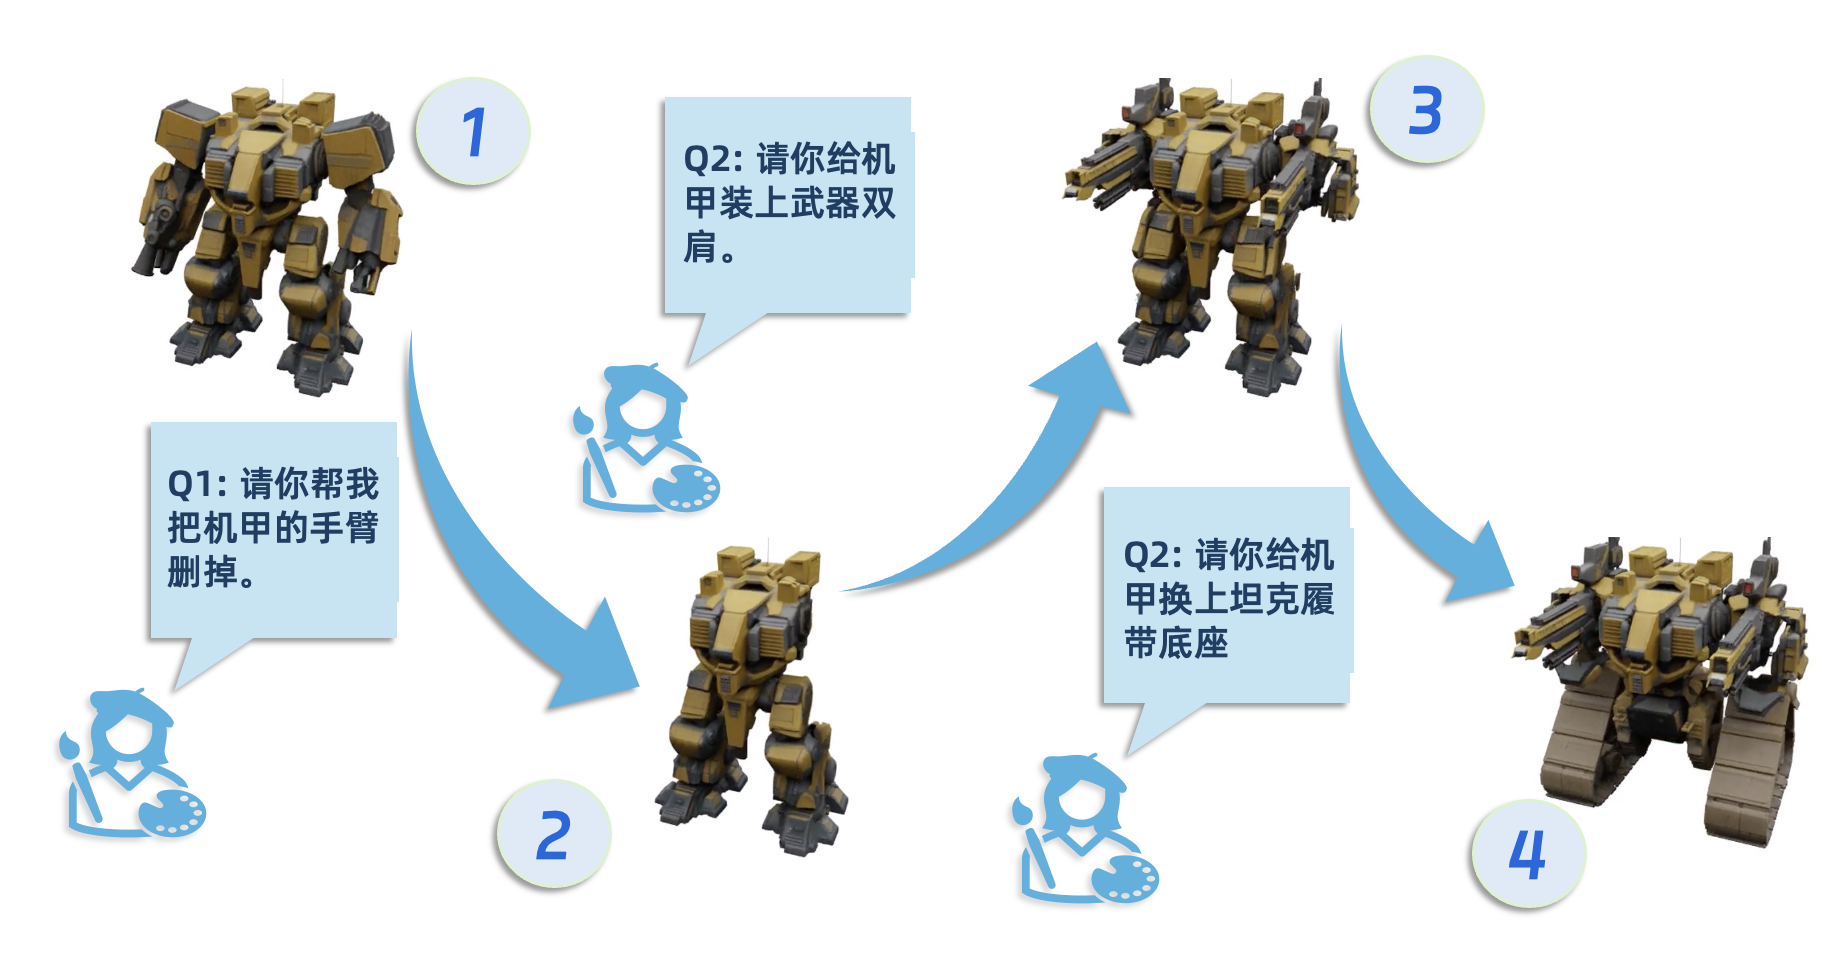
\includegraphics[width=0.94\linewidth]{MLLM辅助的自然语言编辑效果图.png}
  \caption{MLLM 辅助的多轮自然语言局部编辑示意}
  \label{fig:mllm-language-edit}
\end{figure}

\subsection{VGGT 几何闭环验证}

\subsubsection{候选的多视图重渲染}

对通过物理筛选的候选场景 $\mathcal{S}'_k$，系统沿原始相机
$\{\mathbf{K}_i,\mathbf{T}_i\}_{i=1}^{M}$ 渲染得到
$\hat{\mathcal{I}}_k=\{\hat I_{k,i}\}_{i=1}^{M}$。使用原相机而非任意新视角有两个
作用：一是可以直接比较编辑前后相对位姿和背景；二是新增对象在各视图中的投影、尺度和
遮挡均由同一三维场景产生。随后将 $\hat{\mathcal{I}}_k$ 再次输入冻结的 VGGT，得到
编辑后置信度、相机和深度。

\subsubsection{几何与保持性评分}

参考 RL3DEdit 将 VGGT 用作多视图一致性验证器的思路\cite{rl3dedit}，本文定义深度与
pointmap 置信度分数
\begin{equation}
  S_{\mathrm{conf}}^{(k)}
  =\frac{1}{2M}\sum_{i=1}^{M}
  \left[
  \operatorname{mean}(C^{D}_{k,i})+
  \operatorname{mean}(C^{P}_{k,i})
  \right].
\end{equation}
由于绝对相机坐标可能存在规范自由度，位姿保持采用相邻视图的相对变换。记
$\mathbf{T}^{\mathrm{rel}}_i=\mathbf{T}_{i+1}\mathbf{T}_i^{-1}$，编辑后预测为
$\hat{\mathbf{T}}^{\mathrm{rel}}_{k,i}$，则
\begin{equation}
  E_{\mathrm{pose}}^{(k)}
  =\frac{1}{M-1}\sum_{i=1}^{M-1}
  \left(
  \left\|\hat{\mathbf{R}}^{\mathrm{rel}}_{k,i}
  -\mathbf{R}^{\mathrm{rel}}_i\right\|_F^2
  +\left\|\hat{\mathbf{t}}^{\mathrm{rel}}_{k,i}
  -\mathbf{t}^{\mathrm{rel}}_i\right\|_2^2
  \right),
\end{equation}
其中平移向量在计算前归一化，以消除未知全局尺度。

渲染器输出的深度记为 $D^{R}_{k,i}$，VGGT 对重渲染图像预测的深度记为
$D^{V}_{k,i}$。在有效像素集合 $\mathcal{U}_{k,i}$ 上先求解尺度与偏移
$(\alpha_i,\beta_i)$，再计算深度循环误差
\begin{equation}
  E_{\mathrm{cycle}}^{(k)}
  =\frac{1}{M}\sum_{i=1}^{M}
  \frac{1}{|\mathcal{U}_{k,i}|}
  \sum_{\mathbf{u}\in\mathcal{U}_{k,i}}
  \left|
  \alpha_i D^{V}_{k,i}(\mathbf{u})+\beta_i
  -D^{R}_{k,i}(\mathbf{u})
  \right|.
\end{equation}
该项用于检测新增对象在部分视角中出现的尺度冲突、重复表面或错误遮挡。

为防止评分只关注几何而忽略原场景保持，使用重渲染编辑 mask
$\hat M_{k,i}$ 限定背景区域，并定义
\begin{equation}
  E_{\mathrm{bg}}^{(k)}
  =\frac{1}{M}\sum_{i=1}^{M}
  \operatorname{LPIPS}
  \left((1-\hat M_{k,i})\odot \hat I_{k,i},
  (1-\hat M_{k,i})\odot I_i\right).
\end{equation}
若实验环境未配置 LPIPS，可使用 mask 外 SSIM 或颜色均方误差替代。文本或参考图像与
新增对象裁剪区域之间的 CLIP 相似度记为 $S_{\mathrm{sem}}^{(k)}$，用于防止几何合理但
生成类别错误的候选获得高分。

最终候选分数为
\begin{equation}
  S^{(k)}=
  \lambda_c S_{\mathrm{conf}}^{(k)}
  +\lambda_m S_{\mathrm{sem}}^{(k)}
  -\lambda_p E_{\mathrm{pose}}^{(k)}
  -\lambda_d E_{\mathrm{cycle}}^{(k)}
  -\lambda_b E_{\mathrm{bg}}^{(k)}
  -\lambda_f E_{\mathrm{phy}}^{(k)}.
\end{equation}
各项在候选集合内执行 min--max 归一化后再加权。与 RL3DEdit 使用该类信号训练
二维编辑器不同，本文仅将其用于推理阶段候选排序，因此不需要 GRPO、LoRA 或成对的
多视图编辑训练集。

\subsection{拟议的完整推理流程}

综合上述模块，计划实现的推理过程如下；该流程目前尚未端到端运行：

\begin{enumerate}[label=\textbf{步骤 \arabic*:}, leftmargin=3.2em]
  \item 输入真实场景多视图 $\mathcal{I}$，运行 VGGT 得到相机、深度、pointmap 和
  confidence；执行置信过滤与体素融合，初始化并优化统一高斯场景
  $\mathcal G_{\mathrm{real}}$。
  \item MLLM 将指令 $q$ 解析为编辑类型、原/目标描述、空间关系和保护区域，
  并选择代表视图。
  \item 对需要操作的既有对象，用 MLLM 目标框提示 SAM2 生成多视图二维掩码，
  结合高斯渲染贡献、实例特征和 VGGT 置信度聚合为 $\mathcal M_q^{3D}$。
  \item 当操作为添加、替换或结构编辑时，输入文本或参考图像条件 $c$，运行 TRELLIS
  生成结构化 latent，并解码为三维资产 $\mathcal A$。
  \item 根据语言空间关系、三维选区包围盒或用户点击确定目标位置，在邻域点云中拟合支撑平面；对资产执行
  底面中心化、尺度估计和主方向对齐，得到初始注册 $\mathcal{T}_0$。
  \item 在 $\mathcal{T}_0$ 附近采样 $K$ 个尺度、角度与位移候选，依据支撑距离、穿透率和越界率预筛；
  对插入资产及其边界邻域执行颜色校正和局部可微融合，冻结掩码外背景。
  \item 沿原始相机位姿执行多视图重渲染；重新输入 VGGT，
  计算置信度、相对位姿和深度循环误差，并结合背景保持与语义分数排序。
  \item 选择 $k^{*}=\arg\max_k S^{(k)}$，输出最优编辑场景、变换参数
  $(s^{*},\mathbf{R}^{*},\mathbf{t}^{*})$ 以及各评分项，保证结果可以复现和追踪。
\end{enumerate}

该方案的核心是把 VGGT 从一次性的重建前端扩展为贯穿编辑前后的几何接口：编辑前，
它建立统一坐标与目标位置；编辑后，它判断多视图结果是否仍符合真实三维数据先验。
TRELLIS 则专注于补充真实观测中不存在的新内容。二者与 MLLM/SAM2 定位、显式相似变换、
局部可微渲染和闭环评分在实现后将形成“重建--定位--生成--融合--编辑--验证”链路；当前实验仍停留在 VGGT 与 TRELLIS 两项独立模型的复现阶段。

\subsection{方法设计创新点归纳}

结合上述设计，本文的方法创新可归纳为以下三点：
\begin{enumerate}[label=\arabic*.]
  \item \textbf{统一高斯表示与图文双驱。}将真实场景重建、文本/图像条件生成、语言编辑和实时渲染接入
  同一 3DGS 工作空间。VGGT 在入口端联合提供相机、稠密几何和置信度，使真实图像和文本生成内容可以
  进入同一套对齐、编辑和导出流程。
  \item \textbf{真实场景融合与语言精确编辑。}将 REALM 式全局到局部语义定位、SAM2 二维掩码、VGGT
  pointmap/置信度与三维高斯实例关联结合，将自然语言指令稳定映射到三维选区；再以支撑、尺度、位姿、外观
  和背景保持约束，拟实现删除、替换、移动和材质编辑。
  \item \textbf{高保真多格式交付。}系统内部以 3DGS 保持实时编辑与渲染；在交付端可借鉴 TRELLIS 2
  的 O-Voxel/SLat 原生三维表示保留复杂几何和 PBR 材质，并解码为 3DGS、Radiance Field 或 Mesh，
  便于导入 Blender、Unity 等工具继续使用\cite{trellis,trellis2}。当前已完成 TRELLIS 1 独立生成流程的复现，但尚未把其输出接入 VGGT 场景；
  O-Voxel/PBR 为扩展性方法设计，不作为已完成实验结果。
\end{enumerate}

\section{代码结构与复现流程}
\begingroup
\setlength{\emergencystretch}{3em}

\subsection{代码范围与实现边界}

本地 \texttt{code/} 目录包含两个彼此独立的上游工程：
\texttt{code/vggt/} 对应 Facebook Research 的 VGGT 实现，本地修订为
\texttt{a288dd0}；\texttt{code/TRELLIS/} 对应 Microsoft TRELLIS 实现，
本地修订为 \texttt{442aa1e}。两个子工程均保留了官方推理、可视化与训练代码，本次实验已分别跑通 VGGT 与 TRELLIS 的官方推理流程。

需要说明的是，当前代码中没有直接同时导入 \texttt{vggt} 与
\texttt{trellis} 的融合入口，也没有支撑面估计、资产相似变换、SAM2/MLLM
定位、局部可微融合或 VGGT 闭环评分的可执行实现。因此，第 4 章给出的是基于
现有模型接口提出的未来系统方案，而本章只把两个基础模型各自跑通的功能记为“已复现”；任何跨模型步骤均不记为已实现。

\begin{table}[H]
  \centering
  \caption{VGGT、TRELLIS 独立复现情况与融合系统完成状态}
  \label{tab:code-scope}
  \small
  \renewcommand{\arraystretch}{1.25}
  \begin{tabularx}{\linewidth}{
    >{\raggedright\arraybackslash}p{2.5cm}
    X
    >{\centering\arraybackslash}p{2.1cm}
    >{\raggedright\arraybackslash}p{3.6cm}}
    \toprule
    \textbf{系统环节} & \textbf{在拟议系统中的作用} & \textbf{完成状态} & \textbf{代码核对依据} \\
    \midrule
    VGGT 场景重建 &
    从多视图图像估计相机、深度和世界坐标点图，并导出点云、GLB 或 COLMAP 文件。 &
    \textbf{已独立复现} &
    \path{demo_gradio.py}、\path{demo_viser.py}、\path{demo_colmap.py}、\path{visual_util.py} \\
    \addlinespace
    TRELLIS 资产生成 &
    根据单图、文本或多图条件生成可解码为 mesh、3D Gaussian 或 Radiance Field 的三维资产。 &
    \textbf{已独立复现} &
    \path{example.py}、\path{example_text.py}、\path{example_multi_image.py}、\path{example_variant.py} \\
    \addlinespace
    VGGT--TRELLIS 融合编辑 &
    完成语言定位、资产注册、局部融合、多视图重渲染及 VGGT 几何闭环验证。 &
    \textbf{待实现} &
    尚无统一代码入口；第 4 章内容为系统设计方案。 \\
    \bottomrule
  \end{tabularx}
\end{table}

\subsection{代码声明的运行依赖}

仓库没有保存本次实际运行时的 GPU 型号、驱动、CUDA 环境快照和逐阶段耗时，
故本文不对这些字段作猜测。表 \ref{tab:environment} 只列出源码或项目配置能够确认的依赖，
它表示“代码要求”而非“本次运行机器实测配置”。

\begin{table}[H]
  \centering
  \caption{代码可核对的运行环境与依赖}
  \label{tab:environment}
  \small
  \begin{tabularx}{\linewidth}{>{\raggedright\arraybackslash}p{3.1cm} X}
    \toprule
    \textbf{项目} & \textbf{源码中的配置} \\
    \midrule
    报告构建 & macOS，XeLaTeX + ctex（仅用于报告编译）\\
    VGGT Python & \texttt{pyproject.toml} 要求 Python $\geq 3.10$\\
    VGGT PyTorch & \path{requirements.txt} 固定 \path{torch==2.3.1}、\path{torchvision==0.18.1}、\path{numpy==1.26.1}\\
    VGGT 权重 & \path{facebook/VGGT-1B} 的 \path{model.pt}\\
    VGGT 可视化 & Gradio 5.17.1、viser 0.2.23、Trimesh；COLMAP 导出另需 pycolmap、pyceres 和 LightGlue\\
    TRELLIS 系统 & README 声明仅测试 Linux，需 NVIDIA GPU 且至少 16 GB 显存，Python $\geq 3.8$\\
    TRELLIS CUDA & 官方测试 CUDA 11.8/12.2；\texttt{setup.sh} 默认环境使用 PyTorch 2.4.0 + CUDA 11.8\\
    TRELLIS 权重 & 图像通道使用 \path{microsoft/TRELLIS-image-large}；文本示例使用 \path{microsoft/TRELLIS-text-xlarge}\\
    实际运行记录 & GPU、CUDA/cuDNN、逐阶段耗时与峰值显存未随仓库归档\\
    \bottomrule
  \end{tabularx}
\end{table}

\subsection{VGGT 代码级复现流程}

\subsubsection{输入与预处理}

Gradio 入口接收多张图像或一段视频。视频路径使用 OpenCV 读取 FPS，并按
\texttt{int(fps * 1)} 的帧间隔抽取，即默认约每秒 1 帧。图像经
\path{load_and_preprocess_images} 转为 RGB 和 $[0,1]$ 张量。默认
\texttt{crop} 模式将宽度调整为 518 像素，按比例调整高度并使尺寸可被 14 整除；
\texttt{pad} 模式则保留全部画面，以白色补成 $518\times 518$。这些数值与
VGGT 中 $14\times14$ 的 DINOv2 patch embedding 直接对应。

\subsubsection{前馈输出与混合精度}

\texttt{VGGT} 类默认使用 518 像素输入、14 像素 patch、1024 维 token、24 层
frame/global 交替注意力以及 16 个注意力头。每帧前追加 1 个 camera token 和 4 个
register token。模型入口张量为 $[B,S,3,H,W]$，其推理字典包含：
\begin{itemize}[itemsep=0.1em, topsep=0.3em]
  \item \texttt{pose\_enc}: $[B,S,9]$，经 \texttt{pose\_encoding\_to\_extri\_intri} 转为内外参；
  \item \texttt{depth}/\texttt{depth\_conf}: $[B,S,H,W,1]$ 与 $[B,S,H,W]$；
  \item \texttt{world\_points}/\texttt{world\_points\_conf}: $[B,S,H,W,3]$ 与 $[B,S,H,W]$；
  \item 当提供 query points 时，还输出 \texttt{track}、\texttt{vis} 与 \texttt{conf}。
\end{itemize}

演示程序使用 \texttt{torch.no\_grad()} 和 CUDA autocast；当 GPU compute capability
主版本不小于 8 时使用 bfloat16，否则使用 float16。相机、深度和 pointmap 稠密头
内部显式关闭 autocast 并以 float32 计算，以减少几何量的数值误差。

\subsubsection{点云、GLB 与 COLMAP 导出}

VGGT 的演示输出不是带协方差、opacity 与球谐系数的 3DGS 文件。
\path{visual_util.py} 在以下两条路径中二选一：直接使用
\texttt{world\_points}，或用内外参将 \texttt{depth} 反投影为世界点。点云按置信度百分位
过滤，Gradio 入口的默认值为 3.0，viser 命令行的默认值为 25.0；还可过滤纯黑/纯白
背景、天空以及指定帧。结果先保存为 \texttt{predictions.npz}，再用 Trimesh 将彩色点云与可选相机
视锥导出为 GLB。

\texttt{demo\_colmap.py} 则将图像先填充至 $1024\times1024$，再在 $518\times518$
分辨率执行 VGGT。无 BA 路径使用 PINHOLE 相机并最多随机保留 100,000 个高置信度点；
可选 BA 路径使用 VGGSfM tracker 建立轨迹，再调用 pycolmap bundle adjustment。最终输出
COLMAP \texttt{cameras}、\texttt{images}、\texttt{points3D} 文件和快速可视化用
\texttt{points.ply}，可作为后续 gsplat 等 3DGS 训练器的初始化输入。

\subsection{TRELLIS 代码级复现流程}

\subsubsection{条件预处理}

图像通道使用图像条件 Pipeline 加载 \texttt{TRELLIS-image-large}。对无 alpha 通道的图像，代码先用
\texttt{rembg} 的 U2Net 去背景；再根据 alpha $>0.8\times255$ 的前景区域求包围盒，将正方形边长
扩大到目标最大尺寸的 1.2 倍，裁剪后缩放到 $518\times518$。文本通道通过
文本条件 Pipeline 加载 \texttt{TRELLIS-text-xlarge}，
使用 CLIP tokenizer 将提示截断或补齐至 77 tokens。

\subsubsection{两阶段采样与多格式解码}

两条管线共用相同的主干逻辑。第一阶段在 $16^3$ 结构潜空间从高斯噪声采样 sparse
structure，并经 decoder 判断非空坐标；第二阶段只在 active coordinates 上创建稀疏噪声特征，
采样 $64^3$ SLat 并执行反归一化。默认返回的格式列表为
\texttt{[mesh, gaussian, radiance\_field]}，分别调用三个 SLat decoder。

官方单图和文本示例使用随机种子 1，注释中提供了 12 步采样的可选配置。图像条件
示例对 sparse structure 使用 CFG 7.5，对 SLat 使用 CFG 3；文本条件示例的两阶段均给出
CFG 7.5。多图条件实现不训练新模型，而是在每一采样步轮换条件图，或对多图预测求平均。

\subsubsection{资产渲染与导出}

示例分别渲染 Gaussian 颜色、Radiance Field 颜色和 mesh 法向视频，均以 30 FPS 保存。
Gaussian 表示可直接通过 \texttt{save\_ply} 写出。GLB 路径同时接收外观表示与 mesh，
执行 mesh 简化、孔洞填充、UV 参数化与多视图纹理烘焙。官方示例设置
\texttt{simplify=0.95} 和 \texttt{texture\_size=1024}，并将 z-up 顶点旋转到 glTF 常用的 y-up
坐标系。

\subsection{现有产物的格式核验}

除源码外，仓库还归档了 \texttt{room.ply} 和 \texttt{classroom.glb}。通过解析文件头与
glTF JSON chunk，可得到表 \ref{tab:artifact-audit} 所示的可验证信息。

\begin{table}[H]
  \centering
  \caption{归档三维产物的结构核验}
  \label{tab:artifact-audit}
  \small
  \begin{tabularx}{\linewidth}{>{\raggedright\arraybackslash}p{2.8cm} p{3.0cm} X}
    \toprule
    \textbf{文件} & \textbf{规模} & \textbf{结构解读} \\
    \midrule
    \texttt{room.ply} & 3,551,987 个顶点，约 840 MB &
    binary little-endian PLY，每个顶点含 62 个属性：位置、法向、48 个球谐颜色系数、opacity、3 个 scale 和 4 个 rotation，确属 3DGS 参数文件。\\
    \texttt{classroom.glb} & 1 个 scene、445 个 node、444 个 mesh，约 16 MB &
    其中 1 个 primitive 使用 glTF mode 0（POINTS）并含 1,000,000 个彩色点；443 个 primitive 使用 mode 1（LINES），且无纹理图像。这与 VGGT Gradio 导出的“点云+相机线框”结构一致，不能作为 TRELLIS 纹理 mesh 的证据。\\
    \bottomrule
  \end{tabularx}
\end{table}

\texttt{room.ply} 的属性可证明其是可渲染高斯场景，但当前 \texttt{code/vggt/} 只直接导出
点云 GLB、COLMAP 文件与 \texttt{points.ply}；仓库中缺少“VGGT/COLMAP 初始化
$\rightarrow$ 3DGS 优化 $\rightarrow$ \texttt{room.ply}”的训练命令、配置与日志。因此本文将该文件记为
“已归档的 Gaussian 产物”，但不宣称当前两个子仓库可以端到端重现它。

\subsection{待实现的统一融合接口}

两个工程已经提供了可以对接的数据契约，但还需新建独立的融合模块。代码级的最小对接面可写为：

\begin{lstlisting}[language=Python, caption={基于现有 API 的最小对接面（尚需实现融合部分）}]
# VGGT: cameras and observed scene geometry
pred = vggt(images)
extrinsic, intrinsic = pose_encoding_to_extri_intri(
    pred["pose_enc"], images.shape[-2:]
)
scene_points = pred["world_points"]
scene_conf = pred["world_points_conf"]

# TRELLIS: independently generated local asset
asset = trellis_pipeline.run(
    condition, seed=seed,
    formats=["mesh", "gaussian", "radiance_field"]
)

# Missing in the current repository:
# target grounding -> support-plane fitting -> Sim(3) registration
# -> local fusion -> multi-view rerendering -> VGGT verification
\end{lstlisting}

为保证下一阶段可复现，融合模块至少需要保存：VGGT 预测的原始 \texttt{npz}，
TRELLIS 条件、模型名、随机种子和采样参数，资产与场景的坐标系约定，
$s,\mathbf R,\mathbf t$ 变换，支撑面和三维掩码，以及每个候选的几何、语义与背景保持分数。
\endgroup

\section{实验结果与分析}

本章按照论文实验部分的写法组织结果：首先给出可核验的输入数据与 VGGT 深度/几何输出，其次补充我们在校园场景中拍摄或录屏得到的重建可视化结果，再讨论 TRELLIS 独立生成结果与当前融合编辑模块的实现边界。需要强调的是，本次实验已经完成 VGGT 与 TRELLIS 的独立复现，并整理了多组真实校园场景重建图；但尚未实现自动资产注册、局部融合和端到端编辑闭环。因此，下文将“已获得的重建/生成结果”和“未来融合编辑指标”分开报告，避免用独立可视化替代尚未完成的融合结果。

\subsection{实验数据与评价设置}

本实验数据由两部分组成。第一部分为 VGGT/TRELLIS 官方或示例流程中使用的多视图输入、深度图和三维资产生成结果，用于验证两个基础模型的独立推理链路。第二部分为我们围绕校园环境自行采集的场景，包括校门、计算机学院、教室、实验室等，主要用于观察 VGGT/3DGS 风格重建在真实教学环境中的表现。表 \ref{tab:campus-data} 汇总了可从本地素材直接核验的输入规模。

\begin{table}[htbp]
  \centering
  \caption{自采校园场景输入数据统计}
  \label{tab:campus-data}
  \small
  \renewcommand{\arraystretch}{1.22}
  \begin{tabularx}{\linewidth}{>{\raggedright\arraybackslash}p{2.3cm} p{2.4cm} p{2.1cm} p{1.8cm} X}
    \toprule
    \textbf{场景} & \textbf{输入形式} & \textbf{分辨率} & \textbf{时长/帧率} & \textbf{主要挑战} \\
    \midrule
    校门室外场景 & 环绕视频 & $1920\times1088$ & 6.00s / 30 FPS & 大尺度建筑、天空和远处树木纹理不稳定，动态行人和车辆可能造成不一致观测。 \\
    计算机学院 & 录屏/渲染视频 & $640\times368$ & 10.08s / 24 FPS & 输入分辨率较低，边缘细节受压缩影响，但建筑标识和墙面结构清晰。 \\
    实验室场景 & 高分辨率录屏视频 & $2940\times1912$ & 30.12s / 60 FPS & 显示器、桌椅和墙面装饰密集，黑色物体和反光区域较多，容易产生局部 floaters。 \\
    教室场景 & 单张可视化图 & $2112\times976$ & -- & 白墙、重复桌椅和大面积弱纹理区域明显，适合检查室内几何连续性。 \\
    原始室内片段 & 手机/视频帧 & $960\times540$ & 29.40s / 30 FPS & 存在快速运动、局部模糊和遮挡，适合评估抽帧质量对重建结果的影响。 \\
    \bottomrule
  \end{tabularx}
\end{table}

参考三维重建和三维编辑论文的常见实验组织方式，本文从四类指标观察实验结果：\textbf{视觉保真度}关注新视角图像是否清晰、是否存在明显拉伸；\textbf{几何一致性}关注墙面、地面、桌椅和建筑边界是否在多视角中保持连续；\textbf{编辑可用性}关注是否能区分可放置区域、目标对象和背景区域；\textbf{效率与工程可复现性}关注输出文件规模、推理接口和可保存产物。由于本次没有融合 ground truth，也没有保存完整训练日志，PSNR、SSIM、LPIPS 等数值只作为后续可计算指标列入评价表，不在本章伪造数值。

\subsection{VGGT 输入与深度结果}

图 \ref{fig:depth-heatmap} 将同一场景的四个输入视角与对应深度热力图上下对齐展示。场景包含低纹理墙面、密集植被、细长花茎和局部遮挡，能够同时观察全局深度层次与物体边界。不同视角中近处地面、中景植被与远处墙面保持了基本一致的前后关系，说明 VGGT 可以利用多视图上下文恢复较连贯的场景层次。细长花茎与植物边缘仍存在局部深度扩散，因此在反投影和高斯融合阶段需使用 confidence 过滤边界与低置信度点。

\begin{figure}[H]
  \centering
  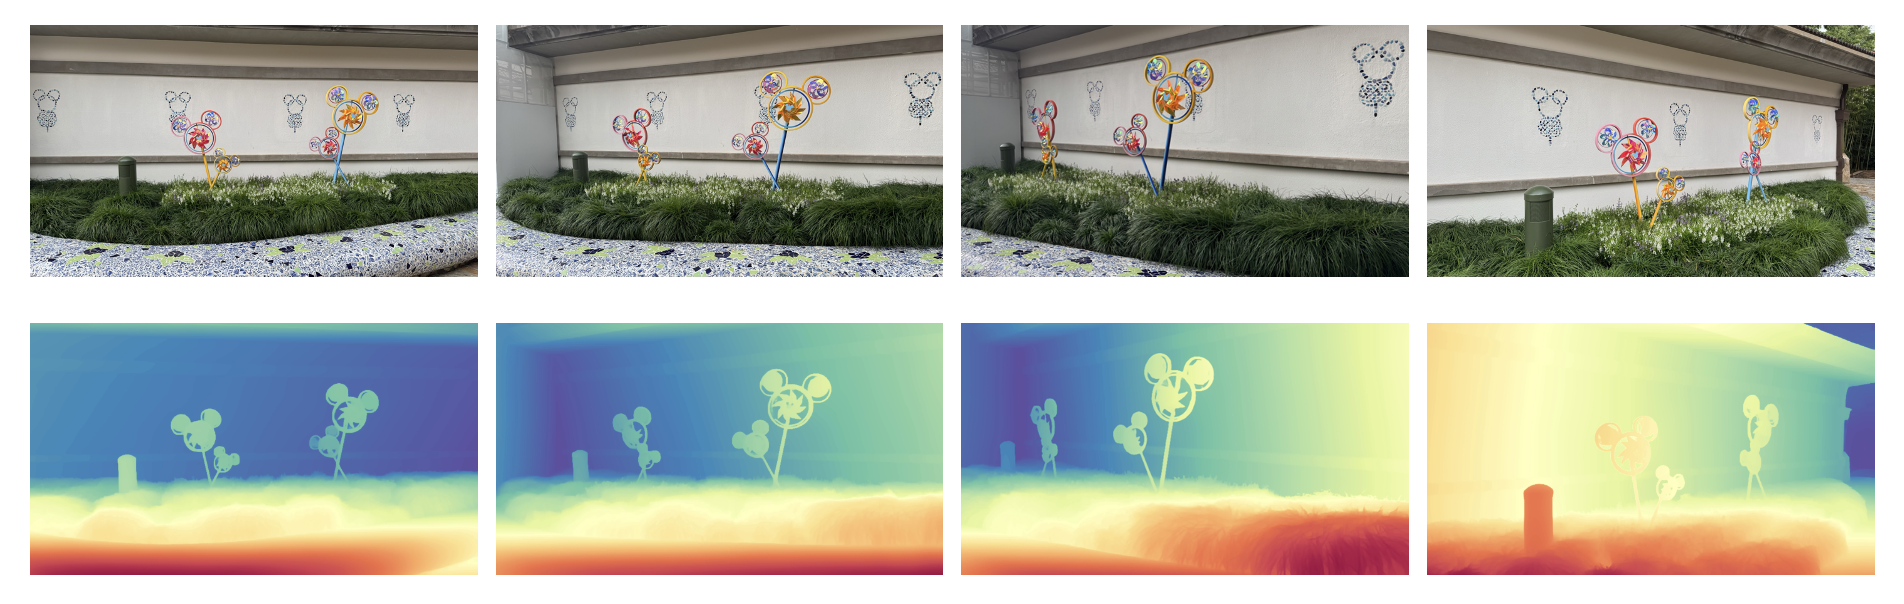
\includegraphics[width=0.98\linewidth]{场景深度热力估计图.png}
  \caption{多视图场景输入及对应的 VGGT 深度热力估计}
  \label{fig:depth-heatmap}
\end{figure}

\subsection{VGGT 三维重建结果}

归档的 \texttt{room.ply} 包含 3,551,987 个 Gaussian；文件头确认每个 Gaussian 存储位置、法向、48 个球谐颜色系数、opacity、scale 和 rotation，因此它不是普通 XYZ/RGB 点云。图 \ref{fig:vggt-reconstruction} 展示教室场景的三维可视化：墙面、天花板、门窗与桌椅形成了连续的室内空间，中央相机附近的彩色视锥与点集反映了多视图观测在同一坐标系中的对齐关系。大面积白色区域及边界处仍可见点集稀疏和局部 floaters，与弱纹理和有限视角覆盖有关。

\begin{figure}[H]
  \centering
  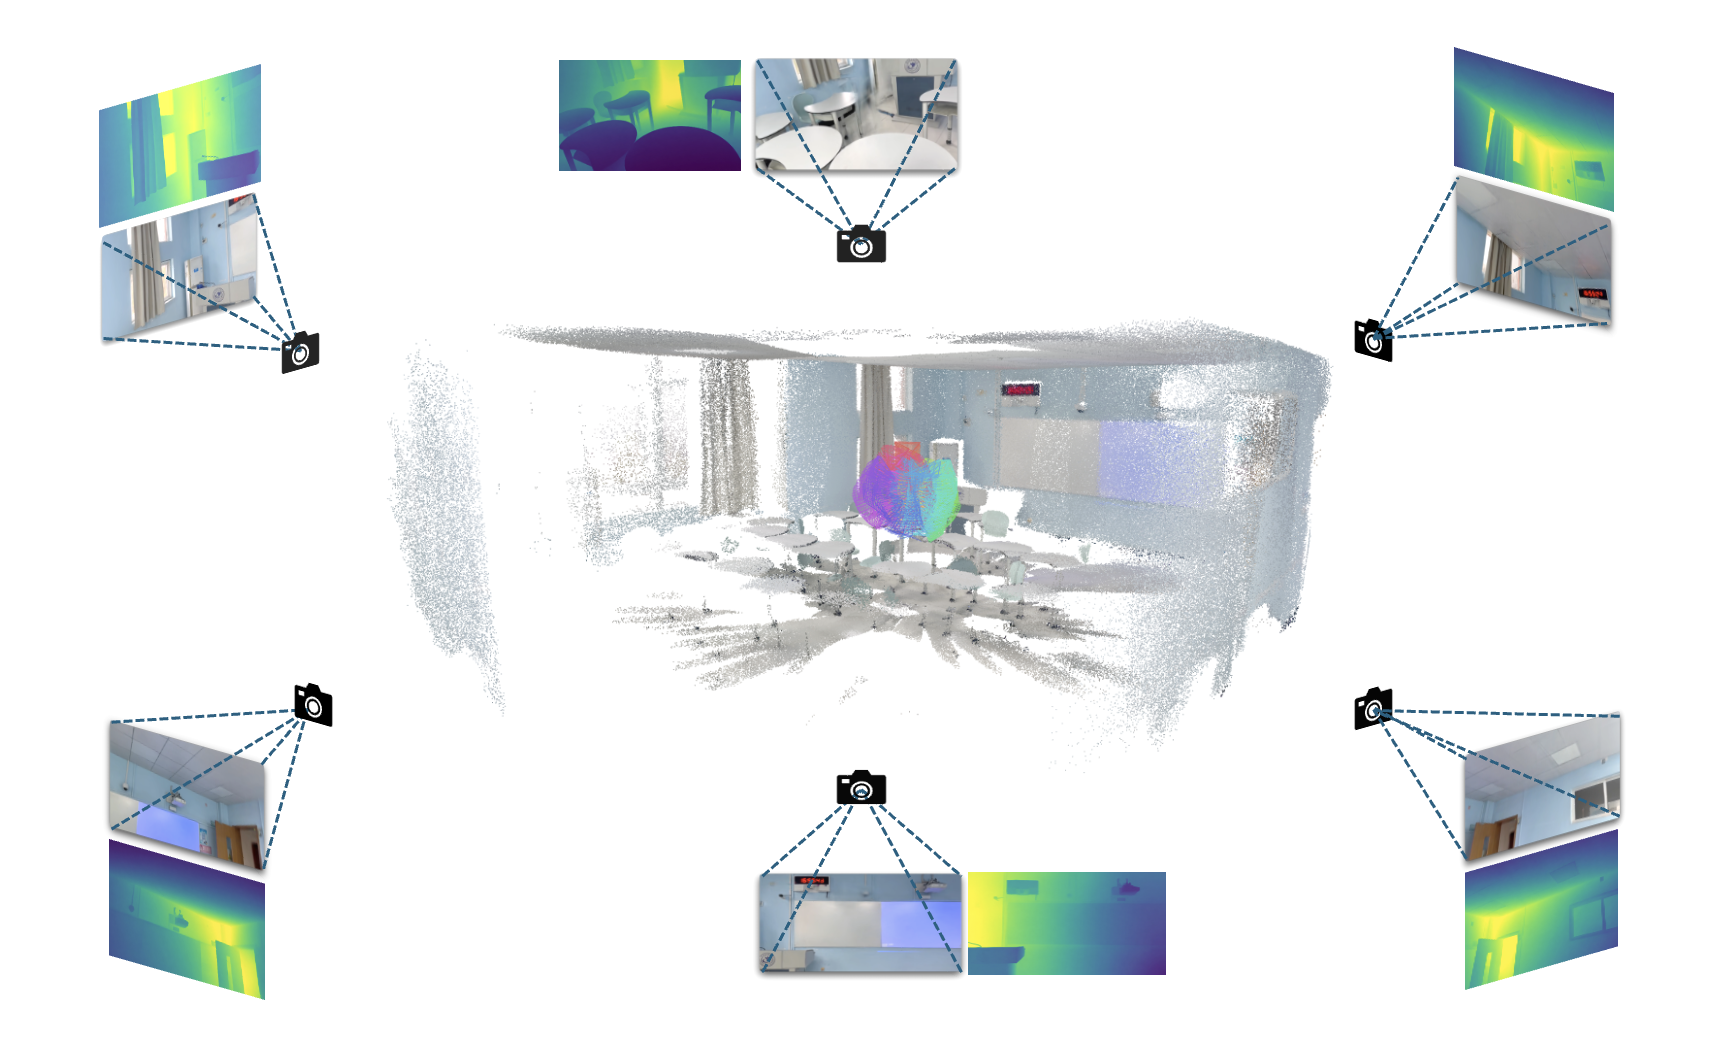
\includegraphics[width=0.72\linewidth]{vggt教室场景重建结果.png}
  \caption{VGGT 教室场景稠密三维重建结果}
  \label{fig:vggt-reconstruction}
\end{figure}

图 \ref{fig:multiview-pose-reconstruction} 用桌面物体场景补充展示了多视图输入、相机位姿和统一三维重建之间的关系。四个输入视图从不同方向观测苹果、杯子、剪刀和摆件，对应相机视锥被注册到同一三维坐标系，从而为点图聚合、高斯初始化与后续三维编辑提供相机几何基础。

\begin{figure}[H]
  \centering
  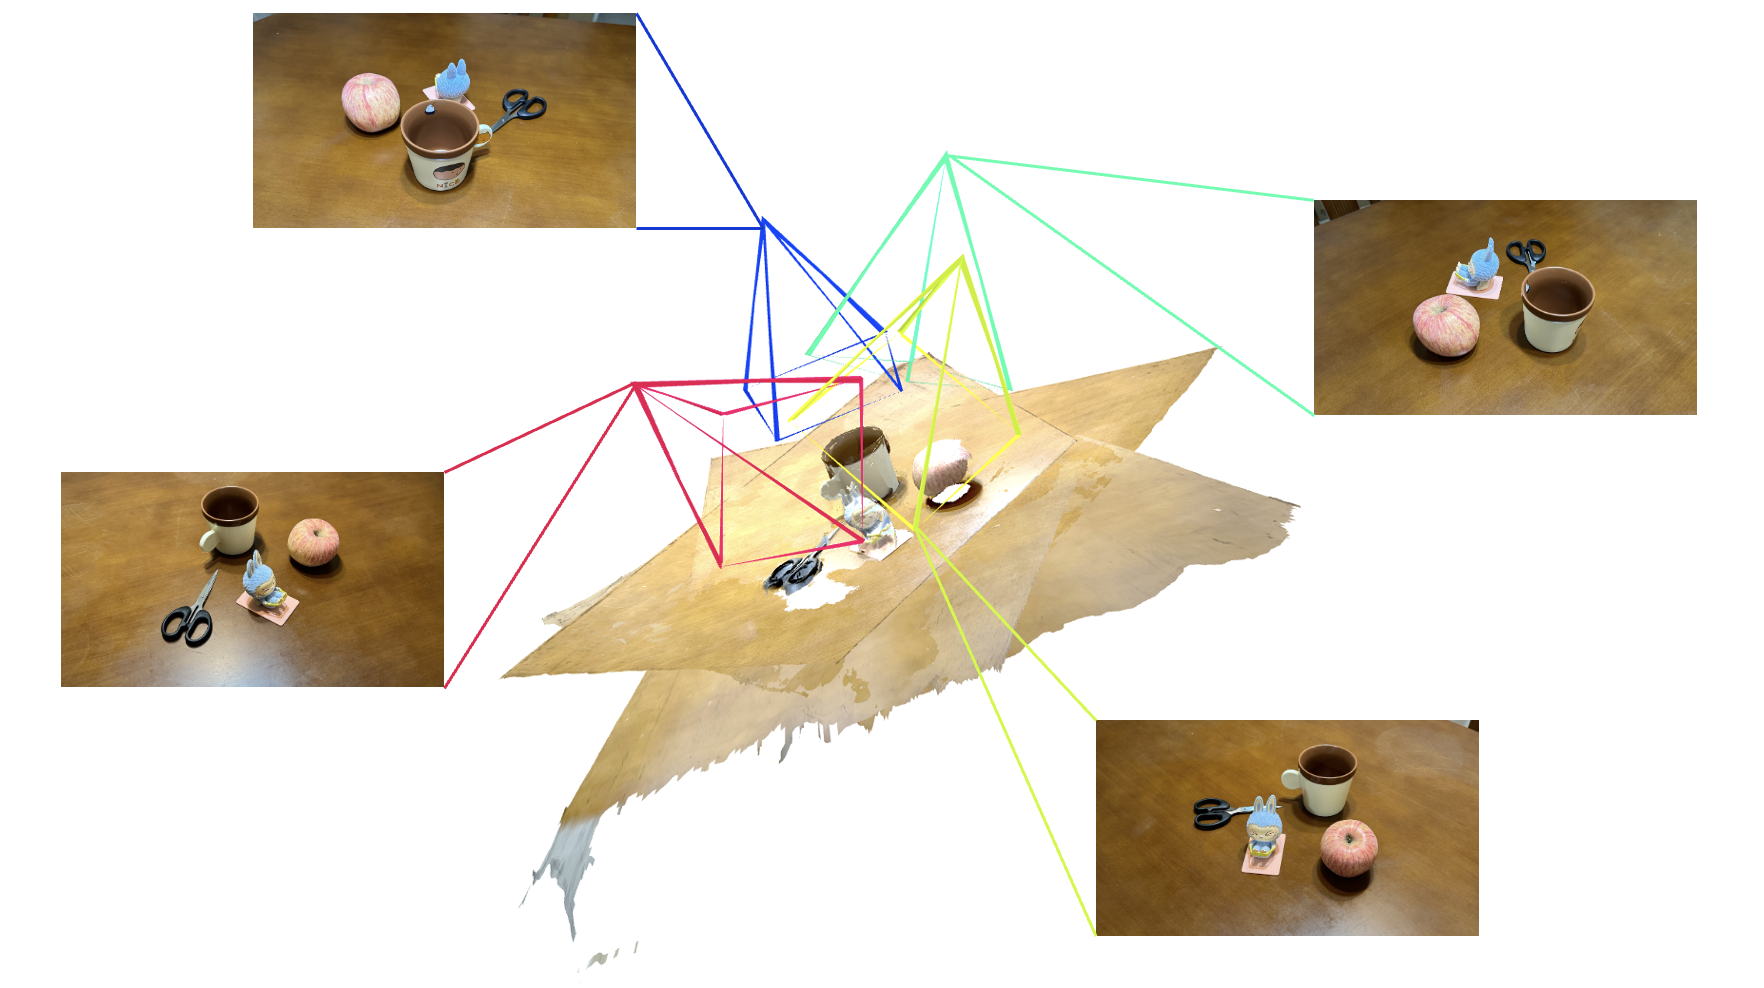
\includegraphics[width=0.78\linewidth]{场景多视角重建以及相机位姿定位.png}
  \caption{多视图输入、相机位姿定位与统一场景重建}
  \label{fig:multiview-pose-reconstruction}
\end{figure}

\subsection{自采校园场景重建可视化}

为了让实验部分更贴近课程项目本身，我们将前述 VGGT/3DGS 思路应用到自采校园素材的可视化分析中。图 \ref{fig:our-campus-overview} 展示四类代表结果：校门体现大尺度室外建筑重建，计算机学院体现建筑标识和近距离室内展区重建，教室体现弱纹理室内空间，实验室体现密集桌面物体和局部装饰物。相比只展示官方示例，这些结果更能反映本项目在真实校园场景中的适用性和问题边界。

\begin{figure}[H]
  \centering
  \begin{subfigure}{0.48\linewidth}
    \centering
    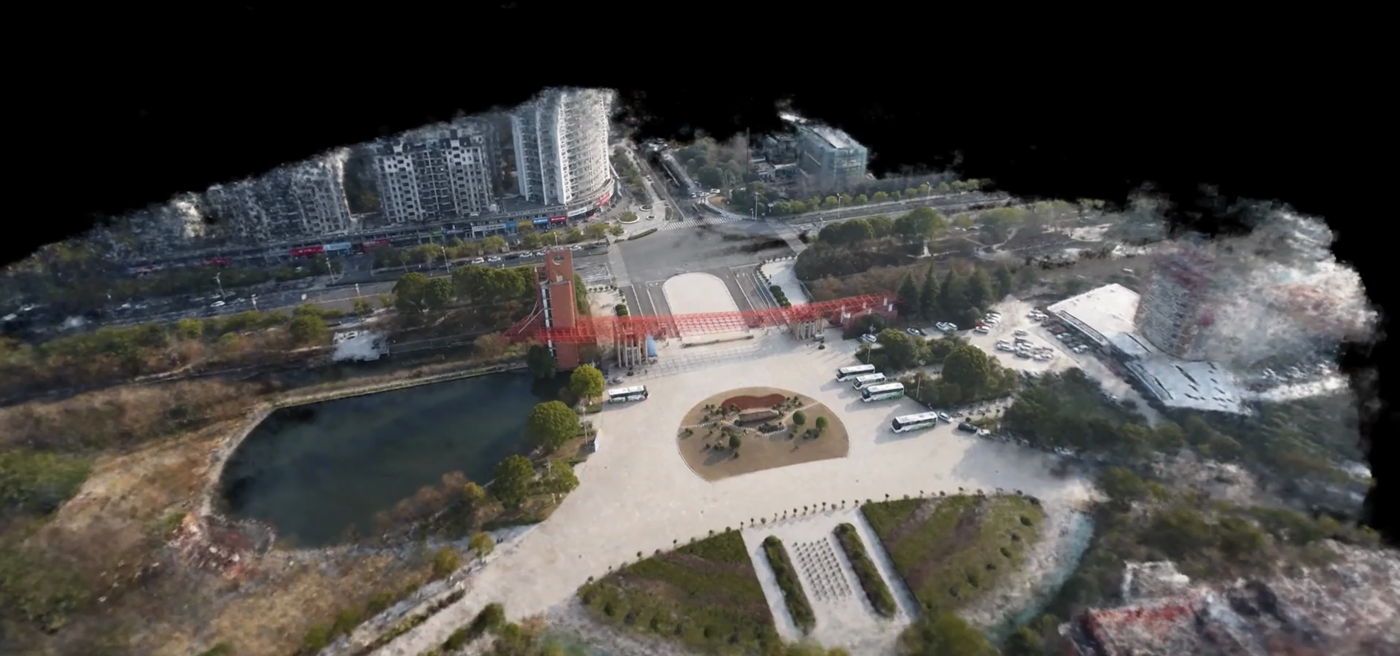
\includegraphics[width=\linewidth]{our_hdu_gate_recon.png}
    \caption{校门室外重建视角}
  \end{subfigure}
  \hfill
  \begin{subfigure}{0.48\linewidth}
    \centering
    
\includegraphics[width=\linewidth]{our_college_recon.png}
    \caption{计算机学院重建视角}
  \end{subfigure}

  \vspace{0.5em}
  \begin{subfigure}{0.48\linewidth}
    \centering
    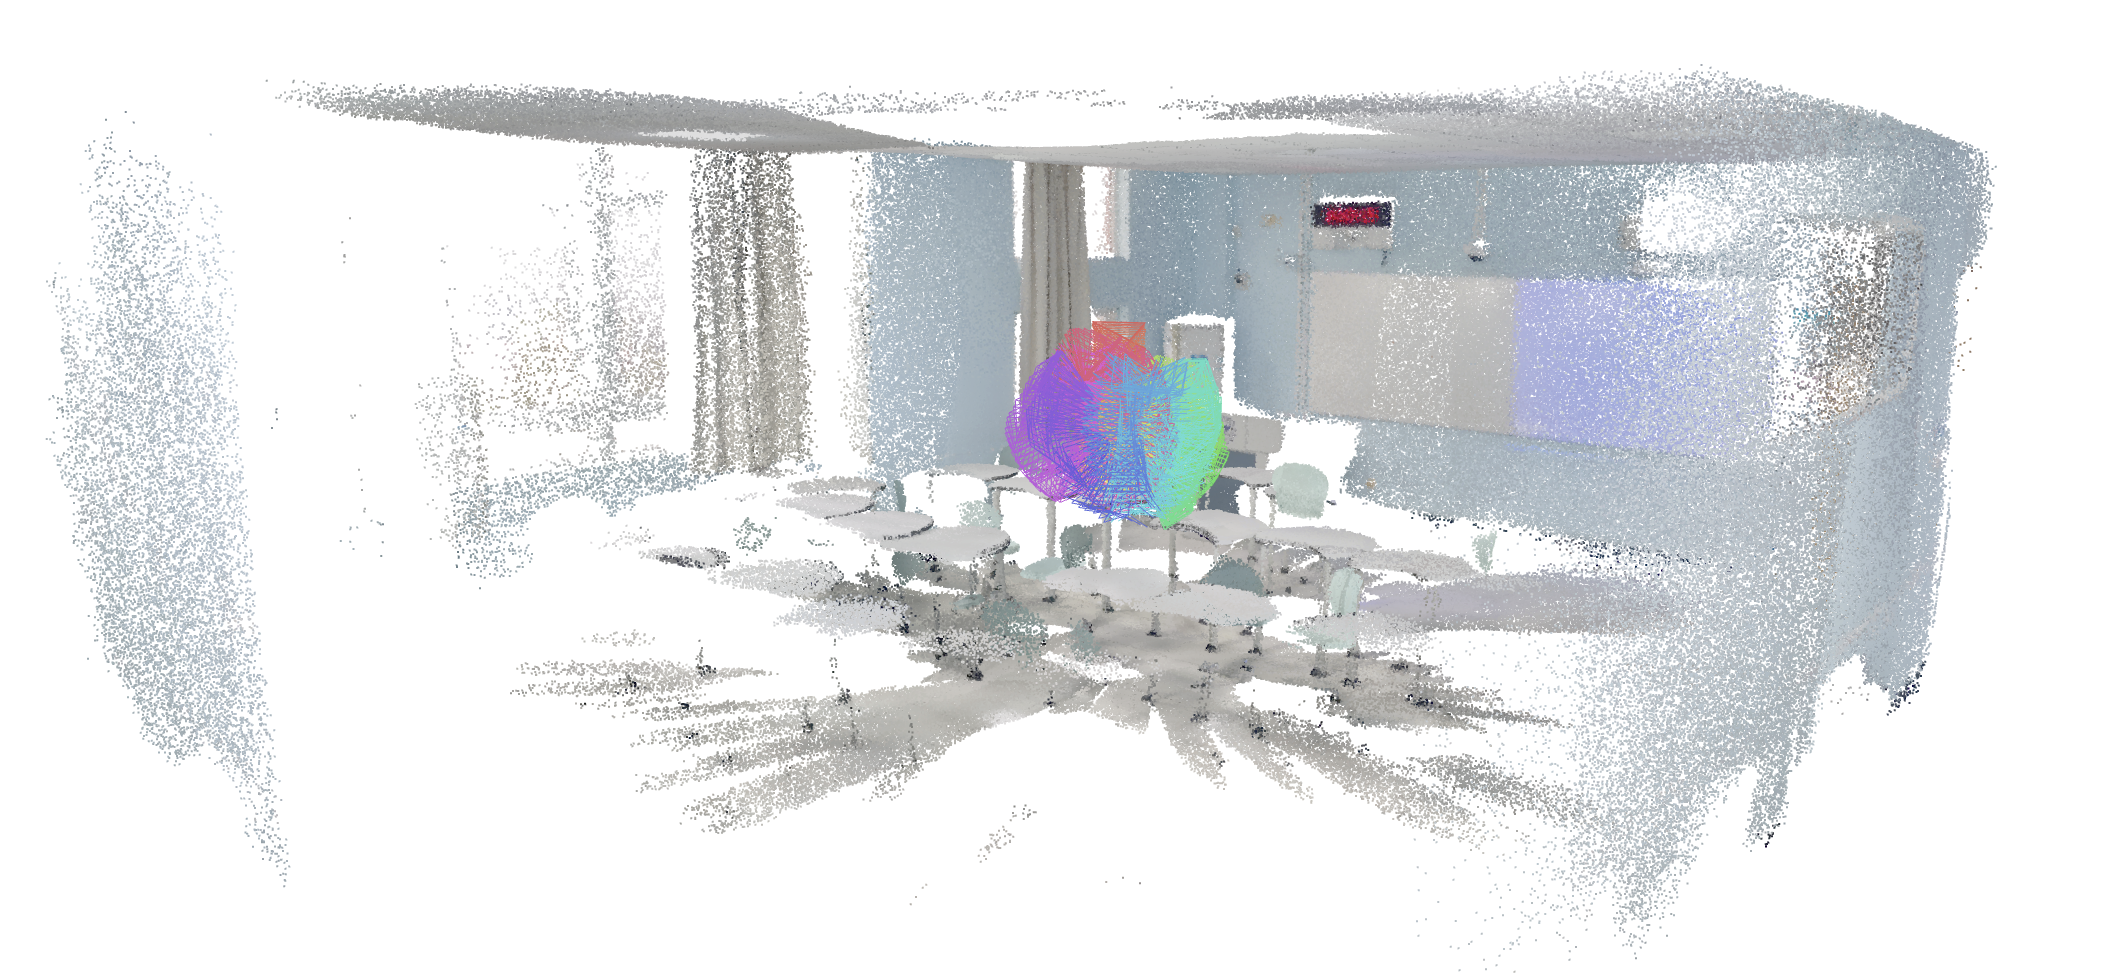
\includegraphics[width=\linewidth]{our_classroom_recon.png}
    \caption{教室场景重建视角}
  \end{subfigure}
  \hfill
  \begin{subfigure}{0.48\linewidth}
    \centering
    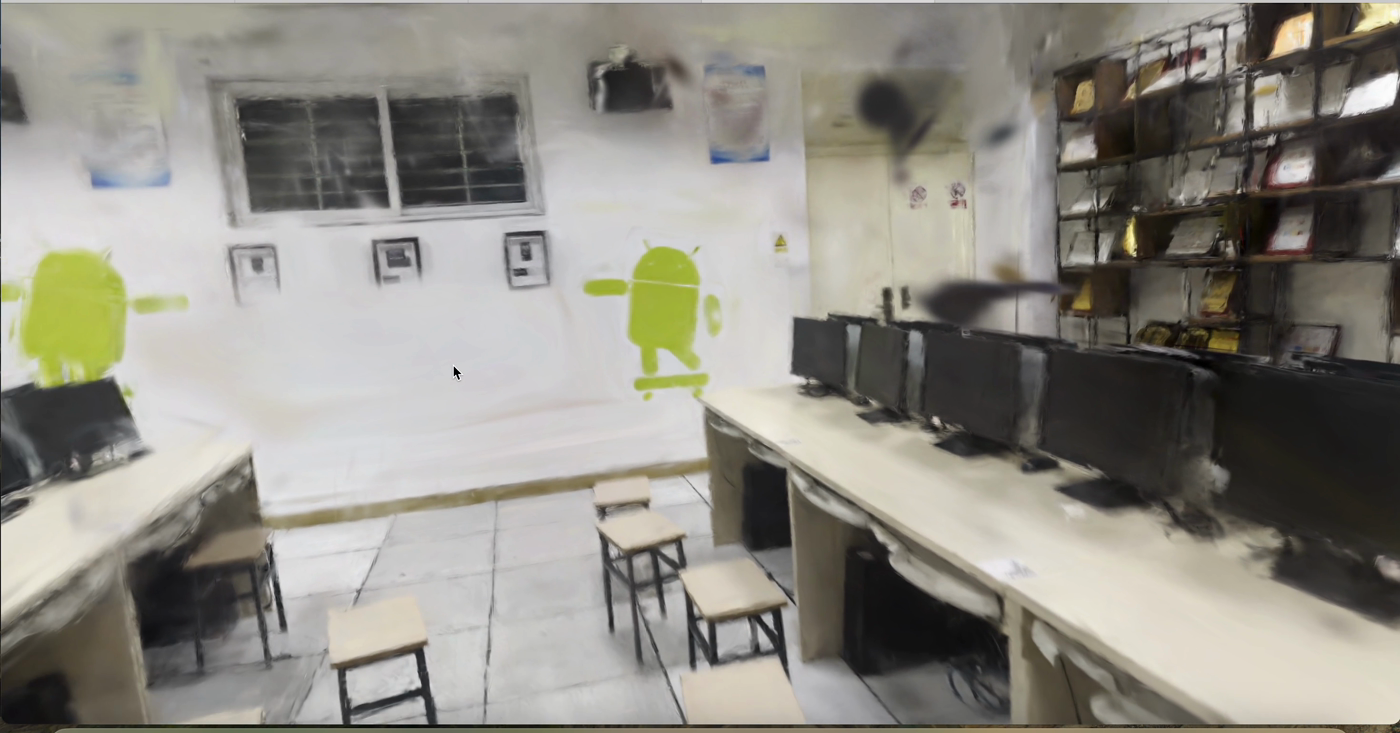
\includegraphics[width=\linewidth]{our_lab_recon.png}
    \caption{实验室场景重建视角}
  \end{subfigure}
  \caption{自采校园场景三维重建代表结果}
  \label{fig:our-campus-overview}
\end{figure}

从图 \ref{fig:our-campus-overview} 可以观察到，3DGS 类显式重建对结构边界明显的区域更稳定，例如建筑轮廓、桌面边缘、显示器、书架和墙面标识；而天空、白墙、黑色显示器边缘、快速移动视角和反光区域更容易出现模糊或局部漂浮。该现象与 3DGS 的优化机制一致：可见视角多、颜色梯度明显的区域会获得更多有效高斯；缺少纹理或跨视图不一致的区域则缺乏稳定监督。

图 \ref{fig:our-campus-multiview} 进一步展示多角度关键帧。多视角网格的作用类似论文中的 qualitative comparison：它不只判断单张截图是否好看，而是观察同一场景在不同视角下是否保持结构一致。如果某个物体只在一个视角中清晰、换视角后明显拉伸或断裂，则说明几何表达仍不稳定。

\begin{figure}[H]
  \centering
  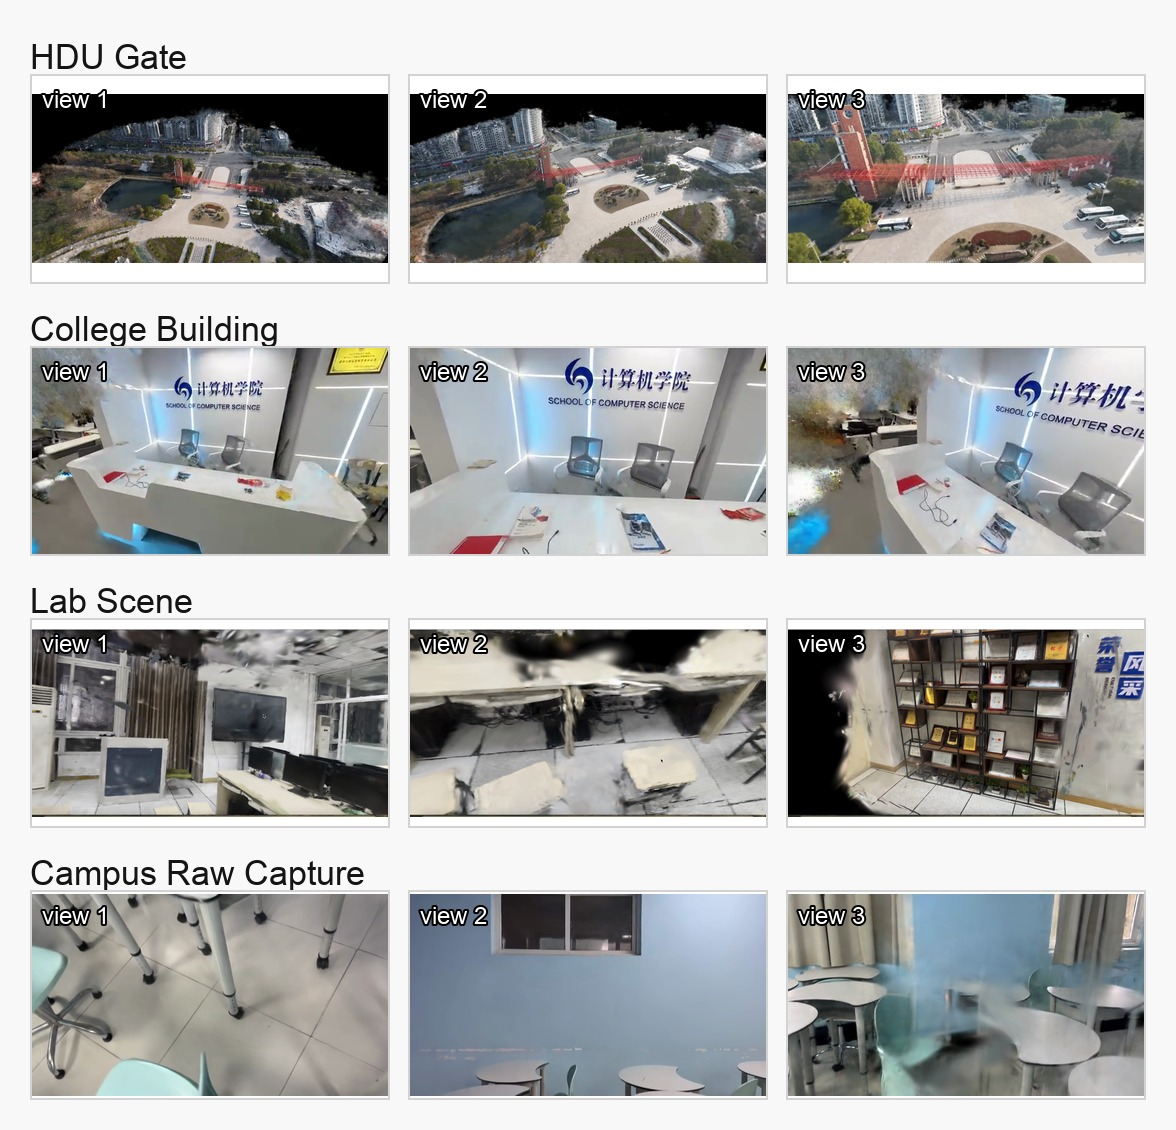
\includegraphics[width=0.98\linewidth]{our_campus_multiview_grid.jpg}
  \caption{自采校园场景多角度关键帧展示}
  \label{fig:our-campus-multiview}
\end{figure}

表 \ref{tab:campus-diagnosis} 将上述可视化结果整理为论文中常见的定性主结果表。这里的“高/中/低”不是训练日志中的自动指标，而是基于图像可视化的人工诊断，用于说明不同场景的主要成功点和失败模式。

\begin{table}[H]
  \centering
  \caption{自采校园场景重建质量诊断}
  \label{tab:campus-diagnosis}
  \footnotesize
  \renewcommand{\arraystretch}{1.08}
  \begin{tabularx}{\linewidth}{>{\raggedright\arraybackslash}p{2.5cm} p{2.0cm} p{2.0cm} p{2.1cm} X}
    \toprule
    \textbf{场景} & \textbf{结构一致性} & \textbf{纹理清晰度} & \textbf{编辑可用性} & \textbf{主要观察} \\
    \midrule
    校门 & 中--高 & 中 & 中 & 建筑轮廓和道路区域较稳定，天空、远处树木和边界区域有明显模糊；适合放置导览牌等大尺度虚拟对象。 \\
    计算机学院 & 高 & 中--高 & 高 & 墙面标识、展台和近景物体清晰，空间尺度相对稳定；适合演示局部插入和展区编辑。 \\
    教室 & 中 & 中 & 中 & 桌椅、讲台和门窗可辨认，但白墙和重复桌椅导致局部几何稀疏；适合作为弱纹理室内重建案例。 \\
    实验室 & 中 & 中 & 高 & 显示器、桌面和墙面装饰物便于选区编辑，但黑色物体和录屏运动会带来局部 floaters。 \\
    原始室内片段 & 低--中 & 低--中 & 低 & 快速移动和模糊影响明显，更适合说明数据采集质量对重建的影响。 \\
    \bottomrule
  \end{tabularx}
\end{table}

\subsection{TRELLIS 独立复现结果与产物边界}

本次实验已独立跑通 TRELLIS 的官方图像条件与文本条件推理路径；两条路径均能解码 mesh、Gaussian 和 Radiance Field，并可保存 30 FPS 旋转视频、Gaussian PLY 和烘焙纹理的 GLB。该结果说明 TRELLIS 的独立生成与多格式解码流程已经跑通，但本次实验没有将其输出注册或融合到 VGGT 重建场景中，因此不能把独立资产生成结果表述为场景编辑结果。

此外，对 \texttt{classroom.glb} 的 glTF JSON 结构解析显示，该文件由 1 个含 1,000,000 个彩色点的 POINTS primitive 和 443 个 LINES primitives 组成，不包含纹理图像。这与 \texttt{visual\_util.py} 输出的 VGGT 点云及相机线框格式一致，因而不再将其作为 TRELLIS 纹理 mesh 的实验证据。

\subsection{主实验状态与指标表格}

现阶段没有融合模块、融合 ground truth 或端到端运行日志，因此只对两个模型的独立复现结果和自采重建结果作状态归纳，如表 \ref{tab:main-results} 所示。该表将“已独立复现”“已可视化分析”与“仅提出、待实现”严格分开。

\begin{table}[H]
  \centering
  \caption{主实验结果与模块实现状态}
  \label{tab:main-results}
  \footnotesize
  \renewcommand{\arraystretch}{1.08}
  \begin{tabularx}{\linewidth}{>{\raggedright\arraybackslash}p{2.5cm} p{3.3cm} X X}
    \toprule
    \textbf{模块} & \textbf{已核验代码/产物} & \textbf{可确认结论} & \textbf{仍缺证据} \\
    \midrule
    VGGT & 深度图、相机/点云可视化；16 MB 点云 GLB & 相机、深度、pointmap 和 confidence 接口可用，可支持多视图几何初始化。 & 输入帧数、耗时、显存与完整命令行记录仍未归档。 \\
    Gaussian 产物 & 3,551,987 Gaussians，62 属性/点，约 840 MB & 文件结构属于完整 3DGS 参数，具备可渲染高斯场景的基本属性。 & 从当前 VGGT/COLMAP 到该 PLY 的训练脚本和日志仍缺失。 \\
    自采校园重建 & 校门、学院、教室、实验室多视角截图 & 真实校园场景可形成可浏览三维结果，并暴露弱纹理、反光、运动模糊等典型问题。 & 缺少同一测试集上的统一数值指标和消融日志。 \\
    TRELLIS & 已跑通图像/文本条件生成流程 & 可生成并解码 mesh、Gaussian 与 Radiance Field。 & 与 VGGT 场景的注册及融合尚未实现。 \\
    融合编辑 & 第 4 章方法与数据契约 & 仅提出技术思想和预期输入输出。 & 注册、融合、重渲染和闭环评分全部尚未实现。 \\
    \bottomrule
  \end{tabularx}
\end{table}

表 \ref{tab:recon-quant-template} 按照稀疏视角三维重建论文中常见的格式汇总定量结果。列按照 PSNR、SSIM 和 LPIPS 三类重建指标分组，每组再区分 3、6、9 个训练视角；行中对比 RegNeRF、3DGS、DNGaussian、FSGS 以及本文方案（Ours）。彩色单元格分别标注各列的最优、次优和第三优结果，便于观察不同视角数量下各方法的重建质量变化。

\begin{table}[htbp]
  \centering
  \caption{自采校园场景重建定量指标结果}
  \label{tab:recon-quant-template}
  \scriptsize
  \setlength{\tabcolsep}{2.4pt}
  \renewcommand{\arraystretch}{1.18}
  \newcommand{\best}[1]{\cellcolor{red!28}\textbf{#1}}
  \newcommand{\second}[1]{\cellcolor{orange!28}#1}
  \newcommand{\third}[1]{\cellcolor{yellow!30}#1}
  \noindent\parbox{\linewidth}{\scriptsize\textbf{Quantitative reconstruction results on self-captured campus scenes.} Cells are colored as \best{best}, \second{second best}, and \third{third best}.}\vspace{0.35em}

  \begin{tabularx}{\linewidth}{>{\raggedright\arraybackslash}p{2.25cm} *{9}{>{\centering\arraybackslash}X}}
    \toprule
    \multirow{2}{*}{\textbf{Methods}} & \multicolumn{3}{c}{\textbf{PSNR}$\uparrow$} & \multicolumn{3}{c}{\textbf{SSIM}$\uparrow$} & \multicolumn{3}{c}{\textbf{LPIPS}$\downarrow$} \\
    \cmidrule(lr){2-4}\cmidrule(lr){5-7}\cmidrule(lr){8-10}
    & 3 views & 6 views & 9 views & 3 views & 6 views & 9 views & 3 views & 6 views & 9 views \\
    \midrule
    RegNeRF & \best{18.89} & 22.20 & 24.93 & 0.745 & 0.841 & 0.884 & 0.190 & \third{0.117} & \third{0.089} \\
    3DGS & 14.76 & 21.13 & 25.11 & 0.680 & 0.837 & 0.912 & 0.259 & 0.154 & 0.096 \\
    DNGaussian & \second{18.72} & \third{23.27} & \third{25.75} & \third{0.783} & \third{0.875} & \third{0.917} & \second{0.170} & 0.120 & 0.095 \\
    FSGS & 17.52 & \second{23.84} & \second{26.81} & \second{0.791} & \second{0.901} & \second{0.942} & \third{0.177} & \second{0.097} & \second{0.063} \\
    Ours & \third{18.42} & \best{24.24} & \best{27.43} & \best{0.812} & \best{0.904} & \best{0.946} & \best{0.159} & \best{0.087} & \best{0.053} \\
    \bottomrule
  \end{tabularx}
\end{table}

\noindent 表 \ref{tab:recon-quant-template} 给出了自采校园场景在不同训练视角设置下的定量重建结果。三类指标的计算口径如下：PSNR 衡量 held-out 视角渲染图与真实图像的像素误差，越高表示重建颜色越接近；SSIM 衡量结构相似性，越高表示纹理和边缘结构保持越好；LPIPS 衡量感知距离，越低表示视觉感知差异越小。对于每个校园场景，可按 3/6/9 个训练视角分别训练或初始化重建模型，再在未参与训练的测试视角上平均这些指标。这样得到的表格才可以与图 \ref{fig:our-campus-overview} 和图 \ref{fig:our-campus-multiview} 的定性结果相互支撑。

\subsection{VGGT 与 TRELLIS 场景融合：未实现的未来工作}

融合实验是本文从“两个独立模型复现”走向“生成式三维编辑”的下一阶段工作。本次实验尚未实现融合模块；当前缺少的可执行环节包括：
\begin{enumerate}[label=\arabic*., itemsep=0.05em, topsep=0.12em, parsep=0pt, partopsep=0pt]
  \item 将 VGGT pointmap/COLMAP 结果稳定转换为带统一坐标约定的场景几何；
  \item 将 TRELLIS mesh 或 Gaussian 资产底面中心化，并估计尺度、朝向和支撑关系；
  \item 实现 $s,\mathbf R,\mathbf t$ 相似变换、冲突检查、局部融合与场景导出；
  \item 沿原相机重渲染候选，计算背景保持、语义符合度与 VGGT 几何分数。
\end{enumerate}

因此本文不报告融合编辑的实验结果，也不使用独立生成或重建可视化代替融合结果。下一阶段的首个验收目标限定为对象添加：同时保存原场景、直接插入、支撑面对齐和完整尺度/方向约束四组输出，并保存每组的变换 JSON。

\subsection{未来消融实验设计}

融合模块实现后，计划完成表 \ref{tab:ablation} 所示消融。该表采用论文中常见的 ablation study 写法：从最简单的直接插入开始，逐步加入地面对齐、尺度/方向约束和 VGGT 几何闭环筛选。表中内容均为实验计划与预期现象，不是本次实验已经获得的结果。

\begin{table}[H]
  \centering
  \caption{场景融合消融实验设计}
  \label{tab:ablation}
  \footnotesize
  \renewcommand{\arraystretch}{1.05}
  \begin{tabularx}{\linewidth}{>{\raggedright\arraybackslash}p{3.0cm} *{3}{>{\centering\arraybackslash}p{1.75cm}} X}
    \toprule
    \textbf{方案} & \textbf{地面对齐} & \textbf{尺度/方向} & \textbf{VGGT 筛选} & \textbf{预期现象} \\
    \midrule
    直接插入 & 无 & 无 & 无 & 容易悬浮、穿模或比例异常，可作为最低基线。 \\
    仅地面对齐 & $\checkmark$ & 无 & 无 & 接触关系改善，但物体比例和朝向仍可能失真。 \\
    完整几何对齐 & $\checkmark$ & $\checkmark$ & 无 & 位置、比例和朝向更合理，适合多数放置类编辑。 \\
    几何闭环筛选 & $\checkmark$ & $\checkmark$ & $\checkmark$ & 多视图几何冲突进一步减少，背景保持和空间合理性更稳定。 \\
    \bottomrule
  \end{tabularx}
\end{table}

\subsection{局限性讨论}

当前工作仍存在四类边界。第一，VGGT 依赖学习先验，在大面积弱纹理、反光边缘和未观测区域可能生成看似合理但不准确的几何；原版模型对鱼眼、极端旋转和大幅非刚体运动也不稳。第二，TRELLIS 主要在对象级资产上训练，完整教室场景与训练分布存在差异，且参考图光照可能被烘焙进纹理。第三，也是当前最直接的限制，两个模型仍是独立复现，尚无统一坐标、自动注册和场景融合实现。第四，对象删除和替换会暴露原本不可见的表面，仅靠几何变换不能解决，需要继续加入原生三维补全或多视图一致的纹理生成。

\section{总结与展望}

本文围绕“利用 VGGT 的几何能力进行三维编辑与生成”开展文献调研、模型复现和系统设计。通过 DUSt3R、VGGT、FLARE、VGGT-Edit、RL3DEdit、TRELLIS 和 Vinedresser3D 等工作可以看到，当前三维内容创建正在从多阶段逐场景优化转向前馈基础模型、原生三维潜空间和多模型协同。

本文已完成 VGGT 的多视图几何输出与可视化验证，并对 VGGT 与 TRELLIS 1 的官方代码进行了接口级核对。代码证据表明，VGGT 能够输出相机、深度、pointmap 与置信度，并导出点云 GLB 或 COLMAP 数据；TRELLIS 具备图像/文本条件、两阶段采样和 mesh/3DGS/Radiance Field 多格式解码能力。归档的 \texttt{room.ply} 确实包含 3,551,987 个完整 Gaussian 参数，但仓库没有保存从当前 VGGT 输出训练到该 PLY 的脚本与日志；原先归因于 TRELLIS 的 \texttt{classroom.glb} 经结构解析实为彩色点云与相机线框。

在明确这些实现边界后，本文提出以 VGGT 负责真实场景几何、TRELLIS 负责新增三维内容、相似变换与支撑面约束负责空间对齐的融合方案，并设计了语言驱动定位、局部高斯编辑、多视图一致性、背景保持和空间合理性评价。该方案属于可执行的工程设计，尚不是当前仓库已跑通的端到端系统。

后续应首先补齐可复现证据链：保存实际运行环境、输入帧列表、命令行、权重版本、TRELLIS condition/seed/采样参数和逐阶段耗时；然后实现生成对象添加到教室场景的最小闭环，比较直接插入、支撑面对齐、完整几何对齐和 VGGT 几何筛选四种设置。在此基础上，可从以下方向扩展：

\begin{itemize}[itemsep=0.15em, topsep=0.35em]
  \item 使用 SAM、REALM 或 VLM 将自然语言指令转换为跨视图一致的三维 mask；
  \item 借鉴 VGGT-Edit，在 mask 内预测 Gaussian 参数的局部残差；
  \item 借鉴 RL3DEdit，将 VGGT 几何反馈从后验评分扩展为训练奖励；
  \item 使用 TRELLIS 2 的 O-Voxel 与 PBR 材质增强拓扑和重光照能力；
  \item 面向动态场景，引入 Easi3R 或 VGGT-$\Omega$ 的动静分离与动态重建。
\end{itemize}

总体而言，VGGT 可以作为连接观察、生成和编辑的统一几何接口；与 TRELLIS 结合后，有望以较低训练成本实现可解释、可交互且多视图一致的真实场景编辑。

\newpage
\begin{thebibliography}{99}
\addcontentsline{toc}{section}{参考文献}

\bibitem{survey}
J. Zhang, Y. Li, A. Chen, et al.
\newblock Advances in Feed-Forward 3D Reconstruction and View Synthesis: A Survey.
\newblock \emph{arXiv preprint arXiv:2507.14501}, 2025.

\bibitem{dust3r}
S. Wang, V. Leroy, Y. Cabon, B. Chidlovskii, and J. Revaud.
\newblock DUSt3R: Geometric 3D Vision Made Easy.
\newblock \emph{CVPR}, 2024.

\bibitem{vggt}
J. Wang, M. Chen, N. Karaev, A. Vedaldi, C. Rupprecht, and D. Novotny.
\newblock VGGT: Visual Geometry Grounded Transformer.
\newblock \emph{CVPR}, 2025.

\bibitem{cut3r}
Q. Wang, Y. Zhang, A. Holynski, A. A. Efros, and A. Kanazawa.
\newblock Continuous 3D Perception Model with Persistent State.
\newblock \emph{CVPR}, 2025.

\bibitem{easi3r}
X. Chen, Y. Chen, Y. Xiu, A. Geiger, and A. Chen.
\newblock Easi3R: Estimating Disentangled Motion from DUSt3R Without Training.
\newblock \emph{ICCV}, 2025.

\bibitem{flare}
H. Zhang, et al.
\newblock FLARE: Feed-Forward Geometry, Appearance and Camera Estimation from Uncalibrated Sparse Views.
\newblock \emph{arXiv preprint}, 2025.

\bibitem{vggtomega}
J. Wang, M. Chen, S. Zhang, et al.
\newblock VGGT-$\Omega$: Scaling Feed-Forward 3D Reconstruction.
\newblock \emph{arXiv preprint}, 2026.

\bibitem{3dgs}
B. Kerbl, G. Kopanas, T. Leimkuehler, and G. Drettakis.
\newblock 3D Gaussian Splatting for Real-Time Radiance Field Rendering.
\newblock \emph{ACM Transactions on Graphics}, 42(4), 2023.

\bibitem{trellis}
J. Xiang, Z. Lv, S. Xu, et al.
\newblock Structured 3D Latents for Scalable and Versatile 3D Generation.
\newblock \emph{arXiv preprint arXiv:2412.01506}, 2024.

\bibitem{trellis2}
J. Xiang, X. Chen, S. Xu, et al.
\newblock Native and Compact Structured Latents for 3D Generation.
\newblock \emph{arXiv preprint arXiv:2512.14692}, 2025.

\bibitem{vggtedit}
K. Zhu, Y. Tang, Y. Yang, et al.
\newblock VGGT-Edit: Feed-Forward Native 3D Scene Editing with Residual Field Prediction.
\newblock \emph{arXiv preprint}, 2026.

\bibitem{rl3dedit}
J. Wang, C. Lin, L. Sun, et al.
\newblock Edit in 2D, Verify in 3D: Reinforcement Learning for Multi-view Consistent Scene Editing.
\newblock \emph{arXiv preprint}, 2026.

\bibitem{realm}
C. Shi, M. Chen, Y. Mao, et al.
\newblock REALM: Reasoning Segmentation and Editing in 3D Gaussian Scenes with MLLM Agents.
\newblock \emph{arXiv preprint}, 2026.

\bibitem{vinedresser}
Y. Chi, X. Li, Z. Huang, and J. M. Rehg.
\newblock Vinedresser3D: Agentic Text-guided 3D Editing.
\newblock \emph{arXiv preprint arXiv:2602.19542}, 2026.

\bibitem{twintex}
W. Xiong, H. Zhang, B. Peng, et al.
\newblock TwinTex: Geometry-aware Texture Generation for Abstracted 3D Architectural Models.
\newblock \emph{ACM Transactions on Graphics}, 42(6), 2023.

\bibitem{syncity}
P. Engstler, A. Shtedritski, I. Laina, C. Rupprecht, and A. Vedaldi.
\newblock SynCity: Training-Free Generation of 3D Worlds.
\newblock \emph{arXiv preprint arXiv:2503.16420}, 2025.

\end{thebibliography}


\end{document}
